\documentclass[twoside]{book}

% Packages required by doxygen
\usepackage{fixltx2e}
\usepackage{calc}
\usepackage{doxygen}
\usepackage[export]{adjustbox} % also loads graphicx
\usepackage{graphicx}
\usepackage[utf8]{inputenc}
\usepackage{makeidx}
\usepackage{multicol}
\usepackage{multirow}
\PassOptionsToPackage{warn}{textcomp}
\usepackage{textcomp}
\usepackage[nointegrals]{wasysym}
\usepackage[table]{xcolor}

% Font selection
\usepackage[T1]{fontenc}
\usepackage[scaled=.90]{helvet}
\usepackage{courier}
\usepackage{amssymb}
\usepackage{sectsty}
\renewcommand{\familydefault}{\sfdefault}
\allsectionsfont{%
  \fontseries{bc}\selectfont%
  \color{darkgray}%
}
\renewcommand{\DoxyLabelFont}{%
  \fontseries{bc}\selectfont%
  \color{darkgray}%
}
\newcommand{\+}{\discretionary{\mbox{\scriptsize$\hookleftarrow$}}{}{}}

% Page & text layout
\usepackage{geometry}
\geometry{%
  a4paper,%
  top=2.5cm,%
  bottom=2.5cm,%
  left=2.5cm,%
  right=2.5cm%
}
\tolerance=750
\hfuzz=15pt
\hbadness=750
\setlength{\emergencystretch}{15pt}
\setlength{\parindent}{0cm}
\setlength{\parskip}{3ex plus 2ex minus 2ex}
\makeatletter
\renewcommand{\paragraph}{%
  \@startsection{paragraph}{4}{0ex}{-1.0ex}{1.0ex}{%
    \normalfont\normalsize\bfseries\SS@parafont%
  }%
}
\renewcommand{\subparagraph}{%
  \@startsection{subparagraph}{5}{0ex}{-1.0ex}{1.0ex}{%
    \normalfont\normalsize\bfseries\SS@subparafont%
  }%
}
\makeatother

% Headers & footers
\usepackage{fancyhdr}
\pagestyle{fancyplain}
\fancyhead[LE]{\fancyplain{}{\bfseries\thepage}}
\fancyhead[CE]{\fancyplain{}{}}
\fancyhead[RE]{\fancyplain{}{\bfseries\leftmark}}
\fancyhead[LO]{\fancyplain{}{\bfseries\rightmark}}
\fancyhead[CO]{\fancyplain{}{}}
\fancyhead[RO]{\fancyplain{}{\bfseries\thepage}}
\fancyfoot[LE]{\fancyplain{}{}}
\fancyfoot[CE]{\fancyplain{}{}}
\fancyfoot[RE]{\fancyplain{}{\bfseries\scriptsize Generated by Doxygen }}
\fancyfoot[LO]{\fancyplain{}{\bfseries\scriptsize Generated by Doxygen }}
\fancyfoot[CO]{\fancyplain{}{}}
\fancyfoot[RO]{\fancyplain{}{}}
\renewcommand{\footrulewidth}{0.4pt}
\renewcommand{\chaptermark}[1]{%
  \markboth{#1}{}%
}
\renewcommand{\sectionmark}[1]{%
  \markright{\thesection\ #1}%
}

% Indices & bibliography
\usepackage{natbib}
\usepackage[titles]{tocloft}
\setcounter{tocdepth}{3}
\setcounter{secnumdepth}{5}
\makeindex

% Hyperlinks (required, but should be loaded last)
\usepackage{ifpdf}
\ifpdf
  \usepackage[pdftex,pagebackref=true]{hyperref}
\else
  \usepackage[ps2pdf,pagebackref=true]{hyperref}
\fi
\hypersetup{%
  colorlinks=true,%
  linkcolor=blue,%
  citecolor=blue,%
  unicode%
}

% Custom commands
\newcommand{\clearemptydoublepage}{%
  \newpage{\pagestyle{empty}\cleardoublepage}%
}

\usepackage{caption}
\captionsetup{labelsep=space,justification=centering,font={bf},singlelinecheck=off,skip=4pt,position=top}

%===== C O N T E N T S =====

\begin{document}

% Titlepage & ToC
\hypersetup{pageanchor=false,
             bookmarksnumbered=true,
             pdfencoding=unicode
            }
\pagenumbering{roman}
\begin{titlepage}
\vspace*{7cm}
\begin{center}%
{\Large C\+SG Tree Point Renderer }\\
\vspace*{1cm}
{\large Generated by Doxygen 1.8.11}\\
\end{center}
\end{titlepage}
\clearemptydoublepage
\tableofcontents
\clearemptydoublepage
\pagenumbering{arabic}
\hypersetup{pageanchor=true}

%--- Begin generated contents ---
\chapter{C\+SG Tree Point Renderer}
\label{md_README}
\hypertarget{md_README}{}
\subsection*{Presentation}


\begin{DoxyItemize}
\item C\+SG + point rendering + random
\item using O\+P\+E\+N\+GL(version ? 3?)/\+G\+L\+UT
\end{DoxyItemize}

\paragraph*{Exemple \+:}







T\+O\+DO constructive solid geometry \href{https://en.wikipedia.org/wiki/Constructive_solid_geometry}{\tt Wikipedia page}.





Other scenes examples are available in directory {\bfseries scenes/}

\subsection*{Usage}


\begin{DoxyItemize}
\item Compilation \+: {\ttfamily make}
\item Run \+: {\ttfamily ./csg scene density}
\begin{DoxyItemize}
\item {\itshape scene} \+: path to the file scene to display
\item {\itshape density} \+: resolution of the scene to display T\+O\+DO V\+A\+L\+UE low, medium, high
\end{DoxyItemize}
\item Delete binaries \+: {\ttfamily make mrproper} 
\end{DoxyItemize}
\chapter{Data Structure Index}
\section{Data Structures}
Here are the data structures with brief descriptions\+:\begin{DoxyCompactList}
\item\contentsline{section}{\hyperlink{struct_node}{Node} \\*Structure defining a C\+SG tree }{\pageref{struct_node}}{}
\item\contentsline{section}{\hyperlink{struct_point_cloud}{Point\+Cloud} \\*Structure defining a point cloud }{\pageref{struct_point_cloud}}{}
\item\contentsline{section}{\hyperlink{struct_shape}{Shape} \\*Structure defining a canonical shape }{\pageref{struct_shape}}{}
\end{DoxyCompactList}

\chapter{File Index}
\section{File List}
Here is a list of all documented files with brief descriptions\+:\begin{DoxyCompactList}
\item\contentsline{section}{include/\hyperlink{parser_8h}{parser.\+h} \\*C\+SG tree parsing module }{\pageref{parser_8h}}{}
\item\contentsline{section}{include/\hyperlink{point__cloud_8h}{point\+\_\+cloud.\+h} \\*Point clound management module }{\pageref{point__cloud_8h}}{}
\item\contentsline{section}{include/\hyperlink{shape_8h}{shape.\+h} \\*Canonical shapes management module }{\pageref{shape_8h}}{}
\item\contentsline{section}{include/\hyperlink{tree_8h}{tree.\+h} \\*C\+SG tree management module }{\pageref{tree_8h}}{}
\item\contentsline{section}{include/\hyperlink{types_8h}{types.\+h} \\*Basic operations management module }{\pageref{types_8h}}{}
\end{DoxyCompactList}

\chapter{Data Structure Documentation}
\hypertarget{struct_node}{}\section{Node Struct Reference}
\label{struct_node}\index{Node@{Node}}


Structure defining a C\+SG tree.  




{\ttfamily \#include $<$tree.\+h$>$}



Collaboration diagram for Node\+:
\nopagebreak
\begin{figure}[H]
\begin{center}
\leavevmode
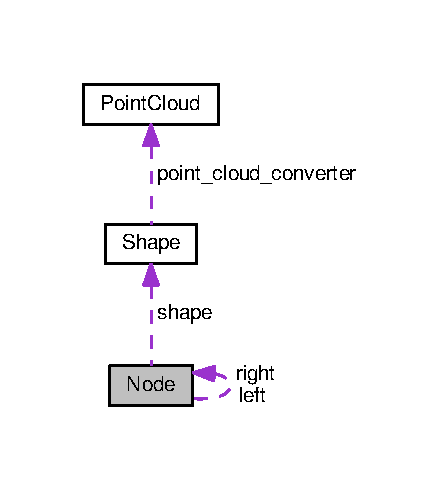
\includegraphics[width=212pt]{struct_node__coll__graph}
\end{center}
\end{figure}
\subsection*{Data Fields}
\begin{DoxyCompactItemize}
\item 
\hyperlink{tree_8h_a7215803e478cdd4bdf4f1b8087cae87b}{Operator} \hyperlink{struct_node_a2a8ef6b2c643a5bc2991ec125cbdb700}{op}
\item 
\hyperlink{struct_shape}{Shape} $\ast$ \hyperlink{struct_node_a3f409da58d3391e8f33c69cce5e4044f}{shape}
\item 
\hyperlink{types_8h_af8defaae7643cbe46b09ad8dea2eca9b}{mat4} \hyperlink{struct_node_aaeb58d722bd66bac7f6f6b4d715ba4c2}{transformations}
\item 
\hyperlink{types_8h_af8defaae7643cbe46b09ad8dea2eca9b}{mat4} \hyperlink{struct_node_a4b726ee7ba7e35b04356dae649a0f39e}{inv\+\_\+transformations}
\item 
\hyperlink{types_8h_af8defaae7643cbe46b09ad8dea2eca9b}{mat4} \hyperlink{struct_node_a902250dd3f3a7dc23af98f9a7df93317}{norm\+\_\+transformations}
\item 
struct \hyperlink{struct_node}{Node} $\ast$ \hyperlink{struct_node_a25eed0b3ce3478a3edb4a00c81dedd5e}{left}
\item 
struct \hyperlink{struct_node}{Node} $\ast$ \hyperlink{struct_node_a760682e46f54442d313a05d18095b52f}{right}
\end{DoxyCompactItemize}


\subsection{Detailed Description}
Structure defining a C\+SG tree. 

A C\+SG tree is a recursive structure. If the tree is a leaf, it is defined by a canonical form. If the tree is an internal node, it is defined by a combination operator, a left C\+SG tree child and a right C\+SG tree child. In both cases, the tree also contains a points transformation matrix, an inverse points transformation matrix, and a normals transformation matrix. 

\subsection{Field Documentation}
\index{Node@{Node}!inv\+\_\+transformations@{inv\+\_\+transformations}}
\index{inv\+\_\+transformations@{inv\+\_\+transformations}!Node@{Node}}
\subsubsection[{\texorpdfstring{inv\+\_\+transformations}{inv_transformations}}]{\setlength{\rightskip}{0pt plus 5cm}{\bf mat4} inv\+\_\+transformations}\hypertarget{struct_node_a4b726ee7ba7e35b04356dae649a0f39e}{}\label{struct_node_a4b726ee7ba7e35b04356dae649a0f39e}
Inverse points transformation matrix \index{Node@{Node}!left@{left}}
\index{left@{left}!Node@{Node}}
\subsubsection[{\texorpdfstring{left}{left}}]{\setlength{\rightskip}{0pt plus 5cm}struct {\bf Node}$\ast$ left}\hypertarget{struct_node_a25eed0b3ce3478a3edb4a00c81dedd5e}{}\label{struct_node_a25eed0b3ce3478a3edb4a00c81dedd5e}
Left C\+SG subtree \index{Node@{Node}!norm\+\_\+transformations@{norm\+\_\+transformations}}
\index{norm\+\_\+transformations@{norm\+\_\+transformations}!Node@{Node}}
\subsubsection[{\texorpdfstring{norm\+\_\+transformations}{norm_transformations}}]{\setlength{\rightskip}{0pt plus 5cm}{\bf mat4} norm\+\_\+transformations}\hypertarget{struct_node_a902250dd3f3a7dc23af98f9a7df93317}{}\label{struct_node_a902250dd3f3a7dc23af98f9a7df93317}
Normals transformation matrix \index{Node@{Node}!op@{op}}
\index{op@{op}!Node@{Node}}
\subsubsection[{\texorpdfstring{op}{op}}]{\setlength{\rightskip}{0pt plus 5cm}{\bf Operator} op}\hypertarget{struct_node_a2a8ef6b2c643a5bc2991ec125cbdb700}{}\label{struct_node_a2a8ef6b2c643a5bc2991ec125cbdb700}
Combination operator \index{Node@{Node}!right@{right}}
\index{right@{right}!Node@{Node}}
\subsubsection[{\texorpdfstring{right}{right}}]{\setlength{\rightskip}{0pt plus 5cm}struct {\bf Node}$\ast$ right}\hypertarget{struct_node_a760682e46f54442d313a05d18095b52f}{}\label{struct_node_a760682e46f54442d313a05d18095b52f}
Right C\+SG subtree \index{Node@{Node}!shape@{shape}}
\index{shape@{shape}!Node@{Node}}
\subsubsection[{\texorpdfstring{shape}{shape}}]{\setlength{\rightskip}{0pt plus 5cm}{\bf Shape}$\ast$ shape}\hypertarget{struct_node_a3f409da58d3391e8f33c69cce5e4044f}{}\label{struct_node_a3f409da58d3391e8f33c69cce5e4044f}
Canonical shape \index{Node@{Node}!transformations@{transformations}}
\index{transformations@{transformations}!Node@{Node}}
\subsubsection[{\texorpdfstring{transformations}{transformations}}]{\setlength{\rightskip}{0pt plus 5cm}{\bf mat4} transformations}\hypertarget{struct_node_aaeb58d722bd66bac7f6f6b4d715ba4c2}{}\label{struct_node_aaeb58d722bd66bac7f6f6b4d715ba4c2}
Points transformation matrix 

The documentation for this struct was generated from the following file\+:\begin{DoxyCompactItemize}
\item 
include/\hyperlink{tree_8h}{tree.\+h}\end{DoxyCompactItemize}

\hypertarget{struct_point_cloud}{}\section{Point\+Cloud Struct Reference}
\label{struct_point_cloud}\index{Point\+Cloud@{Point\+Cloud}}


Structure defining a point cloud.  




{\ttfamily \#include $<$point\+\_\+cloud.\+h$>$}

\subsection*{Data Fields}
\begin{DoxyCompactItemize}
\item 
\hyperlink{types_8h_a5680245085eb6c3661c1ec194979ccd2}{point3} $\ast$ \hyperlink{struct_point_cloud_acc4ce4ac840fff526719963ba4289b8b}{vrtx}
\item 
\hyperlink{types_8h_a1c0f6462cae9caa5b9f49d5ffd32af60}{vec3} $\ast$ \hyperlink{struct_point_cloud_aaa4eb83d6f0f6e7ca1065538784d7de8}{norm}
\item 
\hyperlink{types_8h_a3d75ae93fc87c7ef6399af18de18ed4a}{color4} $\ast$ \hyperlink{struct_point_cloud_a106152c26e8e3dd135a56d7a6431fc9a}{colors}
\item 
int \hyperlink{struct_point_cloud_a439227feff9d7f55384e8780cfc2eb82}{size}
\end{DoxyCompactItemize}


\subsection{Detailed Description}
Structure defining a point cloud. 

A point cloud is defined by a dynamic array of dots, normals and colors. 

\subsection{Field Documentation}
\index{Point\+Cloud@{Point\+Cloud}!colors@{colors}}
\index{colors@{colors}!Point\+Cloud@{Point\+Cloud}}
\subsubsection[{\texorpdfstring{colors}{colors}}]{\setlength{\rightskip}{0pt plus 5cm}{\bf color4}$\ast$ colors}\hypertarget{struct_point_cloud_a106152c26e8e3dd135a56d7a6431fc9a}{}\label{struct_point_cloud_a106152c26e8e3dd135a56d7a6431fc9a}
Colors array \index{Point\+Cloud@{Point\+Cloud}!norm@{norm}}
\index{norm@{norm}!Point\+Cloud@{Point\+Cloud}}
\subsubsection[{\texorpdfstring{norm}{norm}}]{\setlength{\rightskip}{0pt plus 5cm}{\bf vec3}$\ast$ norm}\hypertarget{struct_point_cloud_aaa4eb83d6f0f6e7ca1065538784d7de8}{}\label{struct_point_cloud_aaa4eb83d6f0f6e7ca1065538784d7de8}
Normals array \index{Point\+Cloud@{Point\+Cloud}!size@{size}}
\index{size@{size}!Point\+Cloud@{Point\+Cloud}}
\subsubsection[{\texorpdfstring{size}{size}}]{\setlength{\rightskip}{0pt plus 5cm}int size}\hypertarget{struct_point_cloud_a439227feff9d7f55384e8780cfc2eb82}{}\label{struct_point_cloud_a439227feff9d7f55384e8780cfc2eb82}
Arrays size \index{Point\+Cloud@{Point\+Cloud}!vrtx@{vrtx}}
\index{vrtx@{vrtx}!Point\+Cloud@{Point\+Cloud}}
\subsubsection[{\texorpdfstring{vrtx}{vrtx}}]{\setlength{\rightskip}{0pt plus 5cm}{\bf point3}$\ast$ vrtx}\hypertarget{struct_point_cloud_acc4ce4ac840fff526719963ba4289b8b}{}\label{struct_point_cloud_acc4ce4ac840fff526719963ba4289b8b}
Points array 

The documentation for this struct was generated from the following file\+:\begin{DoxyCompactItemize}
\item 
include/\hyperlink{point__cloud_8h}{point\+\_\+cloud.\+h}\end{DoxyCompactItemize}

\hypertarget{struct_shape}{}\section{Shape Struct Reference}
\label{struct_shape}\index{Shape@{Shape}}


Structure defining a canonical shape.  




{\ttfamily \#include $<$shape.\+h$>$}



Collaboration diagram for Shape\+:
\nopagebreak
\begin{figure}[H]
\begin{center}
\leavevmode
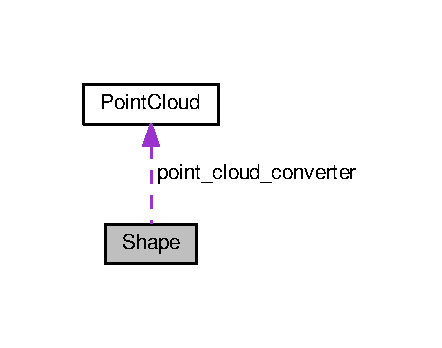
\includegraphics[width=212pt]{struct_shape__coll__graph}
\end{center}
\end{figure}
\subsection*{Data Fields}
\begin{DoxyCompactItemize}
\item 
\hyperlink{shape_8h_a5a4538eeab397888d88a4eefcc5a1345}{Shape\+Type} \hyperlink{struct_shape_aa987badbde9a01a186366bf0bb305a4b}{type}
\item 
\hyperlink{types_8h_a3d75ae93fc87c7ef6399af18de18ed4a}{color4} \hyperlink{struct_shape_a9c2cebcefe8a6bf5fe495236373a6b66}{color}
\item 
double \hyperlink{struct_shape_a9672a1c41e5dd46a6e5f78070594d865}{x\+\_\+scale}
\item 
double \hyperlink{struct_shape_aa03f352193dc2f09d41e8ac49230ca83}{y\+\_\+scale}
\item 
double \hyperlink{struct_shape_abf9d44d8547f49eefd5a5ebf596cb803}{z\+\_\+scale}
\item 
double $\ast$ \hyperlink{struct_shape_a543b882e1acc4b5299df7a74685922db}{args}
\item 
int($\ast$ \hyperlink{struct_shape_afbf4b798f73deb289c638d2204faa656}{contains\+\_\+function} )(double $\ast$, \hyperlink{types_8h_a5680245085eb6c3661c1ec194979ccd2}{point3} $\ast$)
\item 
\hyperlink{struct_point_cloud}{Point\+Cloud} $\ast$($\ast$ \hyperlink{struct_shape_a41118ddb51e72b975315e29488324787}{point\+\_\+cloud\+\_\+converter} )(int, \hyperlink{types_8h_a3d75ae93fc87c7ef6399af18de18ed4a}{color4}, \hyperlink{types_8h_af8defaae7643cbe46b09ad8dea2eca9b}{mat4}, \hyperlink{types_8h_af8defaae7643cbe46b09ad8dea2eca9b}{mat4}, double, double, double, double $\ast$)
\end{DoxyCompactItemize}


\subsection{Detailed Description}
Structure defining a canonical shape. 

Un objet canonique est définit par un type de forme, une couleur, scaling factors, real number arguments (none or several) for parametric shape like torus, a point belonging function, and a conversion function to a point cloud. 

\subsection{Field Documentation}
\index{Shape@{Shape}!args@{args}}
\index{args@{args}!Shape@{Shape}}
\subsubsection[{\texorpdfstring{args}{args}}]{\setlength{\rightskip}{0pt plus 5cm}double$\ast$ args}\hypertarget{struct_shape_a543b882e1acc4b5299df7a74685922db}{}\label{struct_shape_a543b882e1acc4b5299df7a74685922db}
real arguments (for parametric shapes) \index{Shape@{Shape}!color@{color}}
\index{color@{color}!Shape@{Shape}}
\subsubsection[{\texorpdfstring{color}{color}}]{\setlength{\rightskip}{0pt plus 5cm}{\bf color4} color}\hypertarget{struct_shape_a9c2cebcefe8a6bf5fe495236373a6b66}{}\label{struct_shape_a9c2cebcefe8a6bf5fe495236373a6b66}
Color \index{Shape@{Shape}!contains\+\_\+function@{contains\+\_\+function}}
\index{contains\+\_\+function@{contains\+\_\+function}!Shape@{Shape}}
\subsubsection[{\texorpdfstring{contains\+\_\+function}{contains_function}}]{\setlength{\rightskip}{0pt plus 5cm}int($\ast$ contains\+\_\+function) (double $\ast$, {\bf point3} $\ast$)}\hypertarget{struct_shape_afbf4b798f73deb289c638d2204faa656}{}\label{struct_shape_afbf4b798f73deb289c638d2204faa656}
function pointer on the point belonging function \index{Shape@{Shape}!point\+\_\+cloud\+\_\+converter@{point\+\_\+cloud\+\_\+converter}}
\index{point\+\_\+cloud\+\_\+converter@{point\+\_\+cloud\+\_\+converter}!Shape@{Shape}}
\subsubsection[{\texorpdfstring{point\+\_\+cloud\+\_\+converter}{point_cloud_converter}}]{\setlength{\rightskip}{0pt plus 5cm}{\bf Point\+Cloud}$\ast$($\ast$ point\+\_\+cloud\+\_\+converter) (int, {\bf color4}, {\bf mat4}, {\bf mat4}, double, double, double, double $\ast$)}\hypertarget{struct_shape_a41118ddb51e72b975315e29488324787}{}\label{struct_shape_a41118ddb51e72b975315e29488324787}
function pointer on the point cloud conversion function \index{Shape@{Shape}!type@{type}}
\index{type@{type}!Shape@{Shape}}
\subsubsection[{\texorpdfstring{type}{type}}]{\setlength{\rightskip}{0pt plus 5cm}{\bf Shape\+Type} type}\hypertarget{struct_shape_aa987badbde9a01a186366bf0bb305a4b}{}\label{struct_shape_aa987badbde9a01a186366bf0bb305a4b}
Canonical shape type \index{Shape@{Shape}!x\+\_\+scale@{x\+\_\+scale}}
\index{x\+\_\+scale@{x\+\_\+scale}!Shape@{Shape}}
\subsubsection[{\texorpdfstring{x\+\_\+scale}{x_scale}}]{\setlength{\rightskip}{0pt plus 5cm}double x\+\_\+scale}\hypertarget{struct_shape_a9672a1c41e5dd46a6e5f78070594d865}{}\label{struct_shape_a9672a1c41e5dd46a6e5f78070594d865}
Scaling factor on {\itshape x} axis \index{Shape@{Shape}!y\+\_\+scale@{y\+\_\+scale}}
\index{y\+\_\+scale@{y\+\_\+scale}!Shape@{Shape}}
\subsubsection[{\texorpdfstring{y\+\_\+scale}{y_scale}}]{\setlength{\rightskip}{0pt plus 5cm}double y\+\_\+scale}\hypertarget{struct_shape_aa03f352193dc2f09d41e8ac49230ca83}{}\label{struct_shape_aa03f352193dc2f09d41e8ac49230ca83}
Scaling factor on {\itshape y} axis \index{Shape@{Shape}!z\+\_\+scale@{z\+\_\+scale}}
\index{z\+\_\+scale@{z\+\_\+scale}!Shape@{Shape}}
\subsubsection[{\texorpdfstring{z\+\_\+scale}{z_scale}}]{\setlength{\rightskip}{0pt plus 5cm}double z\+\_\+scale}\hypertarget{struct_shape_abf9d44d8547f49eefd5a5ebf596cb803}{}\label{struct_shape_abf9d44d8547f49eefd5a5ebf596cb803}
Scaling factor on {\itshape z} axis 

The documentation for this struct was generated from the following file\+:\begin{DoxyCompactItemize}
\item 
include/\hyperlink{shape_8h}{shape.\+h}\end{DoxyCompactItemize}

\chapter{File Documentation}
\hypertarget{parser_8h}{}\section{include/parser.h File Reference}
\label{parser_8h}\index{include/parser.\+h@{include/parser.\+h}}


C\+SG tree parsing module.  


{\ttfamily \#include \char`\"{}tree.\+h\char`\"{}}\\*
{\ttfamily \#include $<$stdio.\+h$>$}\\*
Include dependency graph for parser.\+h\+:
\nopagebreak
\begin{figure}[H]
\begin{center}
\leavevmode
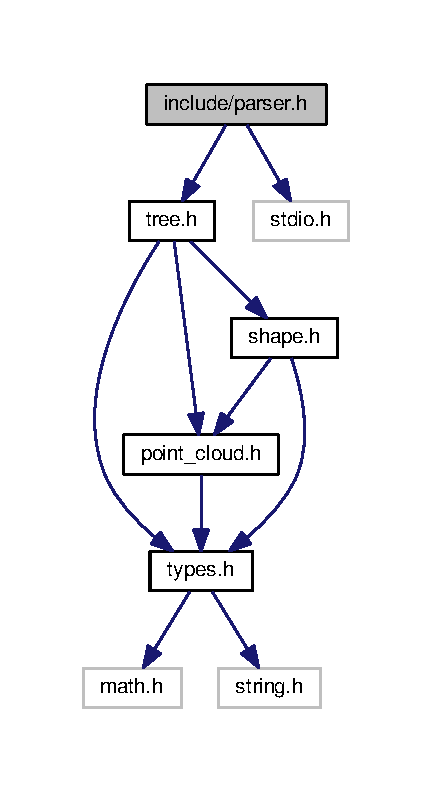
\includegraphics[width=208pt]{parser_8h__incl}
\end{center}
\end{figure}
\subsection*{Macros}
\begin{DoxyCompactItemize}
\item 
\#define \hyperlink{parser_8h_aed906361e2131194a1a5dbf59d26391d}{S\+H\+A\+P\+E\+\_\+\+S\+P\+H\+E\+RE}~(\char`\"{}sphere\char`\"{})\hypertarget{parser_8h_aed906361e2131194a1a5dbf59d26391d}{}\label{parser_8h_aed906361e2131194a1a5dbf59d26391d}

\begin{DoxyCompactList}\small\item\em Sphere token in a scene file. \end{DoxyCompactList}\item 
\#define \hyperlink{parser_8h_ab540250c0c73b3aa9b3dcacdec091b82}{S\+H\+A\+P\+E\+\_\+\+C\+U\+BE}~(\char`\"{}cube\char`\"{})\hypertarget{parser_8h_ab540250c0c73b3aa9b3dcacdec091b82}{}\label{parser_8h_ab540250c0c73b3aa9b3dcacdec091b82}

\begin{DoxyCompactList}\small\item\em Cube token in a scene file. \end{DoxyCompactList}\item 
\#define \hyperlink{parser_8h_abddb505f228469bbe6597b16f02f6e10}{S\+H\+A\+P\+E\+\_\+\+C\+Y\+L\+I\+N\+D\+ER}~(\char`\"{}cylinder\char`\"{})\hypertarget{parser_8h_abddb505f228469bbe6597b16f02f6e10}{}\label{parser_8h_abddb505f228469bbe6597b16f02f6e10}

\begin{DoxyCompactList}\small\item\em Cylinder token in a scene file. \end{DoxyCompactList}\item 
\#define \hyperlink{parser_8h_ae2f671de2e98a442ee8ffe056ca092a1}{S\+H\+A\+P\+E\+\_\+\+C\+O\+NE}~(\char`\"{}cone\char`\"{})\hypertarget{parser_8h_ae2f671de2e98a442ee8ffe056ca092a1}{}\label{parser_8h_ae2f671de2e98a442ee8ffe056ca092a1}

\begin{DoxyCompactList}\small\item\em Cone token in a scene file. \end{DoxyCompactList}\item 
\#define \hyperlink{parser_8h_a46cfff182a5b565663ef6680c6974695}{S\+H\+A\+P\+E\+\_\+\+T\+O\+R\+US}~(\char`\"{}torus\char`\"{})\hypertarget{parser_8h_a46cfff182a5b565663ef6680c6974695}{}\label{parser_8h_a46cfff182a5b565663ef6680c6974695}

\begin{DoxyCompactList}\small\item\em Tore token in a scene file. \end{DoxyCompactList}\item 
\#define \hyperlink{parser_8h_aa237e32e2b19b4c59921efeddca67c79}{O\+P\+E\+R\+A\+T\+O\+R\+\_\+\+I\+D\+E\+N\+T\+I\+TY}~(\char`\"{}=\char`\"{})\hypertarget{parser_8h_aa237e32e2b19b4c59921efeddca67c79}{}\label{parser_8h_aa237e32e2b19b4c59921efeddca67c79}

\begin{DoxyCompactList}\small\item\em Identity operator token in a scene file. \end{DoxyCompactList}\item 
\#define \hyperlink{parser_8h_a6ae34b078004ecd3f89c216c65685bea}{O\+P\+E\+R\+A\+T\+O\+R\+\_\+\+U\+N\+I\+ON}~(\char`\"{}+\char`\"{})\hypertarget{parser_8h_a6ae34b078004ecd3f89c216c65685bea}{}\label{parser_8h_a6ae34b078004ecd3f89c216c65685bea}

\begin{DoxyCompactList}\small\item\em Union operator token in a scene file. \end{DoxyCompactList}\item 
\#define \hyperlink{parser_8h_ad3335be86ab8d79701226a2a55fa19d1}{O\+P\+E\+R\+A\+T\+O\+R\+\_\+\+I\+N\+T\+E\+R\+S\+E\+C\+T\+I\+ON}~(\char`\"{}$\ast$\char`\"{})\hypertarget{parser_8h_ad3335be86ab8d79701226a2a55fa19d1}{}\label{parser_8h_ad3335be86ab8d79701226a2a55fa19d1}

\begin{DoxyCompactList}\small\item\em Intersection operator token in a scene file. \end{DoxyCompactList}\item 
\#define \hyperlink{parser_8h_a2bb8dc3cabc232571dbad6da956179e8}{O\+P\+E\+R\+A\+T\+O\+R\+\_\+\+D\+I\+F\+F\+E\+R\+E\+N\+CE}~(\char`\"{}-\/\char`\"{})\hypertarget{parser_8h_a2bb8dc3cabc232571dbad6da956179e8}{}\label{parser_8h_a2bb8dc3cabc232571dbad6da956179e8}

\begin{DoxyCompactList}\small\item\em Difference operator token in a scene file. \end{DoxyCompactList}\end{DoxyCompactItemize}
\subsection*{Functions}
\begin{DoxyCompactItemize}
\item 
\hyperlink{tree_8h_aa8e9e0ac171efcf72384224fafa0915a}{Tree} \hyperlink{parser_8h_a90c38d4013dd4cb793002cc3ab2b0729}{parse\+\_\+tree} (F\+I\+LE $\ast$file)
\begin{DoxyCompactList}\small\item\em Parse a file to convert it to a C\+SG tree. \end{DoxyCompactList}\end{DoxyCompactItemize}


\subsection{Detailed Description}
C\+SG tree parsing module. 



\subsection{Function Documentation}
\index{parser.\+h@{parser.\+h}!parse\+\_\+tree@{parse\+\_\+tree}}
\index{parse\+\_\+tree@{parse\+\_\+tree}!parser.\+h@{parser.\+h}}
\subsubsection[{\texorpdfstring{parse\+\_\+tree(\+F\+I\+L\+E $\ast$file)}{parse_tree(FILE *file)}}]{\setlength{\rightskip}{0pt plus 5cm}{\bf Tree} parse\+\_\+tree (
\begin{DoxyParamCaption}
\item[{F\+I\+LE $\ast$}]{file}
\end{DoxyParamCaption}
)}\hypertarget{parser_8h_a90c38d4013dd4cb793002cc3ab2b0729}{}\label{parser_8h_a90c38d4013dd4cb793002cc3ab2b0729}


Parse a file to convert it to a C\+SG tree. 

The file must be the result of the depth scan of the tree to be allocated. One line in the file should correspond either to a canonical shape or to a combination operator. Check the readme file for more information on the format to follow. The format must be respected otherwise the program stops.


\begin{DoxyParams}{Parameters}
{\em file} & C\+SG tree file to parse ~\newline
Can not take the value {\itshape N\+U\+LL} \\
\hline
\end{DoxyParams}
\begin{DoxyReturn}{Returns}
the C\+SG tree represented by the file 
\end{DoxyReturn}

\hypertarget{point__cloud_8h}{}\section{include/point\+\_\+cloud.h File Reference}
\label{point__cloud_8h}\index{include/point\+\_\+cloud.\+h@{include/point\+\_\+cloud.\+h}}


Point clound management module.  


{\ttfamily \#include \char`\"{}types.\+h\char`\"{}}\\*
Include dependency graph for point\+\_\+cloud.\+h\+:
\nopagebreak
\begin{figure}[H]
\begin{center}
\leavevmode
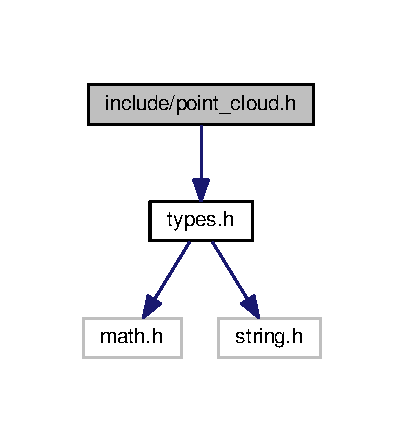
\includegraphics[width=194pt]{point__cloud_8h__incl}
\end{center}
\end{figure}
This graph shows which files directly or indirectly include this file\+:
\nopagebreak
\begin{figure}[H]
\begin{center}
\leavevmode
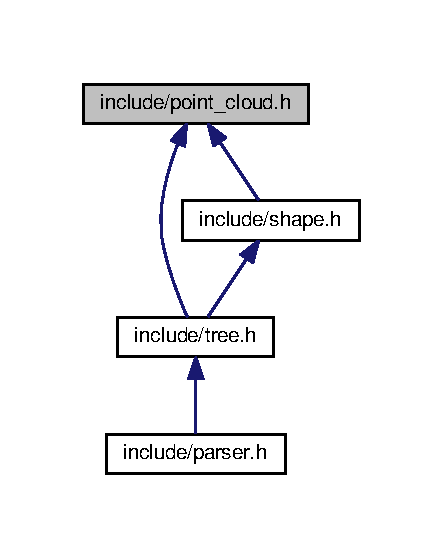
\includegraphics[width=213pt]{point__cloud_8h__dep__incl}
\end{center}
\end{figure}
\subsection*{Data Structures}
\begin{DoxyCompactItemize}
\item 
struct \hyperlink{struct_point_cloud}{Point\+Cloud}
\begin{DoxyCompactList}\small\item\em Structure defining a point cloud. \end{DoxyCompactList}\end{DoxyCompactItemize}
\subsection*{Macros}
\begin{DoxyCompactItemize}
\item 
\#define \hyperlink{point__cloud_8h_a5b748b2b1d95168a4447a233d4cfdf04}{P\+O\+I\+N\+T\+\_\+\+S\+I\+ZE}~(2)\hypertarget{point__cloud_8h_a5b748b2b1d95168a4447a233d4cfdf04}{}\label{point__cloud_8h_a5b748b2b1d95168a4447a233d4cfdf04}

\begin{DoxyCompactList}\small\item\em Size of a point in the point cloud rendering. \end{DoxyCompactList}\end{DoxyCompactItemize}
\subsection*{Functions}
\begin{DoxyCompactItemize}
\item 
\hyperlink{struct_point_cloud}{Point\+Cloud} $\ast$ \hyperlink{point__cloud_8h_a667747d6dab0d1eeba7c51a4452144d1}{point\+\_\+cloud\+\_\+allocate} (\hyperlink{types_8h_a5680245085eb6c3661c1ec194979ccd2}{point3} $\ast$vrtx, \hyperlink{types_8h_a1c0f6462cae9caa5b9f49d5ffd32af60}{vec3} $\ast$norm, \hyperlink{types_8h_a3d75ae93fc87c7ef6399af18de18ed4a}{color4} $\ast$colors, int size)
\begin{DoxyCompactList}\small\item\em Allocate a point cloud. \end{DoxyCompactList}\item 
void \hyperlink{point__cloud_8h_a415c0257d430fe859e38610c909645d4}{point\+\_\+cloud\+\_\+draw} (const \hyperlink{struct_point_cloud}{Point\+Cloud} $\ast$point\+\_\+cloud)
\begin{DoxyCompactList}\small\item\em Draw a point cloud. \end{DoxyCompactList}\item 
void \hyperlink{point__cloud_8h_a229e2722e87922b799ae4b091b98d8a6}{point\+\_\+cloud\+\_\+free} (\hyperlink{struct_point_cloud}{Point\+Cloud} $\ast$$\ast$point\+\_\+cloud)
\begin{DoxyCompactList}\small\item\em Free the memory allocated by a point cloud. \end{DoxyCompactList}\item 
int \hyperlink{point__cloud_8h_aba5b30dd25a089751d4394e93408e0d8}{point\+\_\+cloud\+\_\+is\+\_\+valid} (const \hyperlink{struct_point_cloud}{Point\+Cloud} $\ast$point\+\_\+cloud)
\begin{DoxyCompactList}\small\item\em Test if a point cloud datastructure is valid. \end{DoxyCompactList}\end{DoxyCompactItemize}


\subsection{Detailed Description}
Point clound management module. 



\subsection{Function Documentation}
\index{point\+\_\+cloud.\+h@{point\+\_\+cloud.\+h}!point\+\_\+cloud\+\_\+allocate@{point\+\_\+cloud\+\_\+allocate}}
\index{point\+\_\+cloud\+\_\+allocate@{point\+\_\+cloud\+\_\+allocate}!point\+\_\+cloud.\+h@{point\+\_\+cloud.\+h}}
\subsubsection[{\texorpdfstring{point\+\_\+cloud\+\_\+allocate(point3 $\ast$vrtx, vec3 $\ast$norm, color4 $\ast$colors, int size)}{point_cloud_allocate(point3 *vrtx, vec3 *norm, color4 *colors, int size)}}]{\setlength{\rightskip}{0pt plus 5cm}{\bf Point\+Cloud}$\ast$ point\+\_\+cloud\+\_\+allocate (
\begin{DoxyParamCaption}
\item[{{\bf point3} $\ast$}]{vrtx, }
\item[{{\bf vec3} $\ast$}]{norm, }
\item[{{\bf color4} $\ast$}]{colors, }
\item[{int}]{size}
\end{DoxyParamCaption}
)}\hypertarget{point__cloud_8h_a667747d6dab0d1eeba7c51a4452144d1}{}\label{point__cloud_8h_a667747d6dab0d1eeba7c51a4452144d1}


Allocate a point cloud. 

Arrays in parameters must absolutely be dynamically allocated. They will be released when the point cloud is released. The arrays should have the same size. The program stops if the allocation has failed.


\begin{DoxyParams}{Parameters}
{\em vrtx} & Points array ~\newline
Can not take the value {\itshape N\+U\+LL} \\
\hline
{\em norm} & Normals array ~\newline
Can not take the value {\itshape N\+U\+LL} \\
\hline
{\em colors} & Colors array ~\newline
Can not take the value {\itshape N\+U\+LL} \\
\hline
{\em size} & Arrays size ~\newline
Must be strictly positive\\
\hline
\end{DoxyParams}
\begin{DoxyReturn}{Returns}
a pointer to the allocated point cloud 
\end{DoxyReturn}
\index{point\+\_\+cloud.\+h@{point\+\_\+cloud.\+h}!point\+\_\+cloud\+\_\+draw@{point\+\_\+cloud\+\_\+draw}}
\index{point\+\_\+cloud\+\_\+draw@{point\+\_\+cloud\+\_\+draw}!point\+\_\+cloud.\+h@{point\+\_\+cloud.\+h}}
\subsubsection[{\texorpdfstring{point\+\_\+cloud\+\_\+draw(const Point\+Cloud $\ast$point\+\_\+cloud)}{point_cloud_draw(const PointCloud *point_cloud)}}]{\setlength{\rightskip}{0pt plus 5cm}void point\+\_\+cloud\+\_\+draw (
\begin{DoxyParamCaption}
\item[{const {\bf Point\+Cloud} $\ast$}]{point\+\_\+cloud}
\end{DoxyParamCaption}
)}\hypertarget{point__cloud_8h_a415c0257d430fe859e38610c909645d4}{}\label{point__cloud_8h_a415c0257d430fe859e38610c909645d4}


Draw a point cloud. 


\begin{DoxyParams}{Parameters}
{\em point\+\_\+cloud} & Point cloud to draw ~\newline
Can not take the value {\itshape N\+U\+LL} ~\newline
Must be a valid point cloud \\
\hline
\end{DoxyParams}
\index{point\+\_\+cloud.\+h@{point\+\_\+cloud.\+h}!point\+\_\+cloud\+\_\+free@{point\+\_\+cloud\+\_\+free}}
\index{point\+\_\+cloud\+\_\+free@{point\+\_\+cloud\+\_\+free}!point\+\_\+cloud.\+h@{point\+\_\+cloud.\+h}}
\subsubsection[{\texorpdfstring{point\+\_\+cloud\+\_\+free(\+Point\+Cloud $\ast$$\ast$point\+\_\+cloud)}{point_cloud_free(PointCloud **point_cloud)}}]{\setlength{\rightskip}{0pt plus 5cm}void point\+\_\+cloud\+\_\+free (
\begin{DoxyParamCaption}
\item[{{\bf Point\+Cloud} $\ast$$\ast$}]{point\+\_\+cloud}
\end{DoxyParamCaption}
)}\hypertarget{point__cloud_8h_a229e2722e87922b799ae4b091b98d8a6}{}\label{point__cloud_8h_a229e2722e87922b799ae4b091b98d8a6}


Free the memory allocated by a point cloud. 

Arrays will also be deallocated and the pointed point cloud will be set to {\itshape N\+U\+LL}.


\begin{DoxyParams}{Parameters}
{\em point\+\_\+cloud} & Pointer to the point cloud to free ~\newline
Can not take the value {\itshape N\+U\+LL} Must be a valid point cloud \\
\hline
\end{DoxyParams}
\index{point\+\_\+cloud.\+h@{point\+\_\+cloud.\+h}!point\+\_\+cloud\+\_\+is\+\_\+valid@{point\+\_\+cloud\+\_\+is\+\_\+valid}}
\index{point\+\_\+cloud\+\_\+is\+\_\+valid@{point\+\_\+cloud\+\_\+is\+\_\+valid}!point\+\_\+cloud.\+h@{point\+\_\+cloud.\+h}}
\subsubsection[{\texorpdfstring{point\+\_\+cloud\+\_\+is\+\_\+valid(const Point\+Cloud $\ast$point\+\_\+cloud)}{point_cloud_is_valid(const PointCloud *point_cloud)}}]{\setlength{\rightskip}{0pt plus 5cm}int point\+\_\+cloud\+\_\+is\+\_\+valid (
\begin{DoxyParamCaption}
\item[{const {\bf Point\+Cloud} $\ast$}]{point\+\_\+cloud}
\end{DoxyParamCaption}
)}\hypertarget{point__cloud_8h_aba5b30dd25a089751d4394e93408e0d8}{}\label{point__cloud_8h_aba5b30dd25a089751d4394e93408e0d8}


Test if a point cloud datastructure is valid. 

A point cloud is valid if \+: ~\newline

\begin{DoxyItemize}
\item {\bfseries size} is strictly positive ~\newline

\item {\bfseries vrtx} is different from {\itshape N\+U\+LL} ~\newline

\item {\bfseries norm} is different from {\itshape N\+U\+LL} ~\newline

\item {\bfseries colors} is different from {\itshape N\+U\+LL} 
\end{DoxyItemize}


\begin{DoxyParams}{Parameters}
{\em point\+\_\+cloud} & Point cloud to test ~\newline
Can not take the value {\itshape N\+U\+LL} \\
\hline
\end{DoxyParams}
\begin{DoxyReturn}{Returns}
{\itshape 1} if the point cloud is valid, {\itshape 0} otherwise 
\end{DoxyReturn}

\hypertarget{shape_8h}{}\section{include/shape.h File Reference}
\label{shape_8h}\index{include/shape.\+h@{include/shape.\+h}}


Canonical shapes management module.  


{\ttfamily \#include \char`\"{}types.\+h\char`\"{}}\\*
{\ttfamily \#include \char`\"{}point\+\_\+cloud.\+h\char`\"{}}\\*
Include dependency graph for shape.\+h\+:
\nopagebreak
\begin{figure}[H]
\begin{center}
\leavevmode
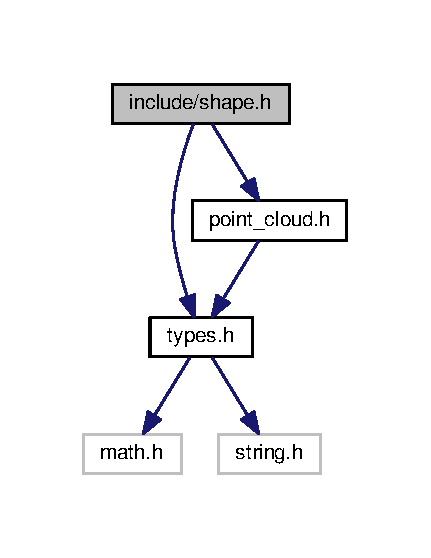
\includegraphics[width=207pt]{shape_8h__incl}
\end{center}
\end{figure}
This graph shows which files directly or indirectly include this file\+:
\nopagebreak
\begin{figure}[H]
\begin{center}
\leavevmode
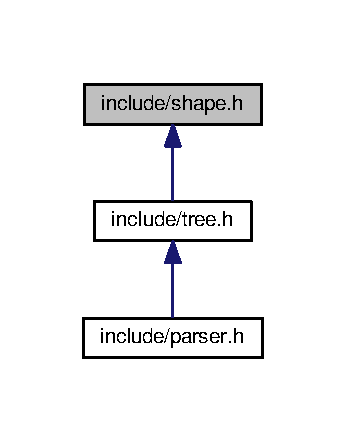
\includegraphics[width=166pt]{shape_8h__dep__incl}
\end{center}
\end{figure}
\subsection*{Data Structures}
\begin{DoxyCompactItemize}
\item 
struct \hyperlink{struct_shape}{Shape}
\begin{DoxyCompactList}\small\item\em Structure defining a canonical shape. \end{DoxyCompactList}\end{DoxyCompactItemize}
\subsection*{Enumerations}
\begin{DoxyCompactItemize}
\item 
enum \hyperlink{shape_8h_a5a4538eeab397888d88a4eefcc5a1345}{Shape\+Type} \{ \\*
\hyperlink{shape_8h_a5a4538eeab397888d88a4eefcc5a1345a3b4c5831cd0a4399644876494915540a}{Sphere}, 
\hyperlink{shape_8h_a5a4538eeab397888d88a4eefcc5a1345a9a0ac0e1bcb1e95a77ef54d9f6658337}{Cube}, 
\hyperlink{shape_8h_a5a4538eeab397888d88a4eefcc5a1345ad35bd028b7dd1821600a81852499e66e}{Cylinder}, 
\hyperlink{shape_8h_a5a4538eeab397888d88a4eefcc5a1345a6bf79fd4474dc6d32585a80411b9e30e}{Cone}, 
\\*
\hyperlink{shape_8h_a5a4538eeab397888d88a4eefcc5a1345abab368199df5c1742ff025831e085ea2}{Torus}, 
\hyperlink{shape_8h_a5a4538eeab397888d88a4eefcc5a1345a136b0b9b9a840b2bfbfeb3da97d6895c}{Number\+Shape\+Type}
 \}\begin{DoxyCompactList}\small\item\em Enumeration of the different types of canonical shapes available. \end{DoxyCompactList}
\end{DoxyCompactItemize}
\subsection*{Functions}
\begin{DoxyCompactItemize}
\item 
\hyperlink{struct_point_cloud}{Point\+Cloud} $\ast$ \hyperlink{shape_8h_a1561f8b563792a2b4b4ffa4c00b14782}{shape\+\_\+to\+\_\+point\+\_\+cloud} (const \hyperlink{struct_shape}{Shape} $\ast$shape, int density, \hyperlink{types_8h_af8defaae7643cbe46b09ad8dea2eca9b}{mat4} transformations, \hyperlink{types_8h_af8defaae7643cbe46b09ad8dea2eca9b}{mat4} norm\+\_\+transformations)
\begin{DoxyCompactList}\small\item\em Convert a canonical shape to a point cloud. \end{DoxyCompactList}\item 
\hyperlink{struct_shape}{Shape} $\ast$ \hyperlink{shape_8h_a8ddd9b9df081a8826e95f4c21812b358}{shape\+\_\+cone} (\hyperlink{types_8h_a3d75ae93fc87c7ef6399af18de18ed4a}{color4} color)
\begin{DoxyCompactList}\small\item\em Allocate a canonical cone. \end{DoxyCompactList}\item 
\hyperlink{struct_shape}{Shape} $\ast$ \hyperlink{shape_8h_a544e890bea51d0c03dd15bc9ef7ef53c}{shape\+\_\+cube} (\hyperlink{types_8h_a3d75ae93fc87c7ef6399af18de18ed4a}{color4} color)
\begin{DoxyCompactList}\small\item\em Allocate a canonical cube. \end{DoxyCompactList}\item 
int \hyperlink{shape_8h_ad41d41c7f11e39bc118b2fb68d33a4e3}{shape\+\_\+contains\+\_\+point} (const \hyperlink{struct_shape}{Shape} $\ast$shape, const \hyperlink{types_8h_a5680245085eb6c3661c1ec194979ccd2}{point3} $\ast$point)
\begin{DoxyCompactList}\small\item\em Test if a point belongs to a canonical shape. \end{DoxyCompactList}\item 
\hyperlink{struct_shape}{Shape} $\ast$ \hyperlink{shape_8h_ad6897ba7aad8581b826054866fc8392e}{shape\+\_\+cylinder} (\hyperlink{types_8h_a3d75ae93fc87c7ef6399af18de18ed4a}{color4} color)
\begin{DoxyCompactList}\small\item\em Allocate a canonical cylinder. \end{DoxyCompactList}\item 
void \hyperlink{shape_8h_a0523f8c3f6929bf27c9f9a5158fdd926}{shape\+\_\+free} (\hyperlink{struct_shape}{Shape} $\ast$$\ast$shape)
\begin{DoxyCompactList}\small\item\em Free the memory allocated by a canonical shape. \end{DoxyCompactList}\item 
int \hyperlink{shape_8h_a75610191099f8f54de836b5492a6a159}{shape\+\_\+is\+\_\+valid} (const \hyperlink{struct_shape}{Shape} $\ast$shape)
\begin{DoxyCompactList}\small\item\em Test if a canonical shape datastructure is valid. \end{DoxyCompactList}\item 
void \hyperlink{shape_8h_a5977cbf2428b20d5b20d9b9a78067b44}{shape\+\_\+rescale} (\hyperlink{struct_shape}{Shape} $\ast$shape, double x, double y, double z)
\begin{DoxyCompactList}\small\item\em Perform a scaling on a canonical shape. \end{DoxyCompactList}\item 
\hyperlink{struct_shape}{Shape} $\ast$ \hyperlink{shape_8h_a2bcca475ad0946dbee15d87acd8425ad}{shape\+\_\+sphere} (\hyperlink{types_8h_a3d75ae93fc87c7ef6399af18de18ed4a}{color4} color)
\begin{DoxyCompactList}\small\item\em Allocate a canonical sphere. \end{DoxyCompactList}\item 
\hyperlink{struct_shape}{Shape} $\ast$ \hyperlink{shape_8h_add89074e3ba5f35e8fd2161f441aea70}{shape\+\_\+torus} (\hyperlink{types_8h_a3d75ae93fc87c7ef6399af18de18ed4a}{color4} color, double radius)
\begin{DoxyCompactList}\small\item\em Allocate a canonical torus. \end{DoxyCompactList}\end{DoxyCompactItemize}


\subsection{Detailed Description}
Canonical shapes management module. 



\subsection{Enumeration Type Documentation}
\index{shape.\+h@{shape.\+h}!Shape\+Type@{Shape\+Type}}
\index{Shape\+Type@{Shape\+Type}!shape.\+h@{shape.\+h}}
\subsubsection[{\texorpdfstring{Shape\+Type}{ShapeType}}]{\setlength{\rightskip}{0pt plus 5cm}enum {\bf Shape\+Type}}\hypertarget{shape_8h_a5a4538eeab397888d88a4eefcc5a1345}{}\label{shape_8h_a5a4538eeab397888d88a4eefcc5a1345}


Enumeration of the different types of canonical shapes available. 

This information is not essential but can be useful to make statistics on the C\+SG tree, like for example to count the number of cube in the scene. \begin{Desc}
\item[Enumerator]\par
\begin{description}
\index{Sphere@{Sphere}!shape.\+h@{shape.\+h}}\index{shape.\+h@{shape.\+h}!Sphere@{Sphere}}\item[{\em 
Sphere\hypertarget{shape_8h_a5a4538eeab397888d88a4eefcc5a1345a3b4c5831cd0a4399644876494915540a}{}\label{shape_8h_a5a4538eeab397888d88a4eefcc5a1345a3b4c5831cd0a4399644876494915540a}
}]Canonical sphere \index{Cube@{Cube}!shape.\+h@{shape.\+h}}\index{shape.\+h@{shape.\+h}!Cube@{Cube}}\item[{\em 
Cube\hypertarget{shape_8h_a5a4538eeab397888d88a4eefcc5a1345a9a0ac0e1bcb1e95a77ef54d9f6658337}{}\label{shape_8h_a5a4538eeab397888d88a4eefcc5a1345a9a0ac0e1bcb1e95a77ef54d9f6658337}
}]Canonical cube \index{Cylinder@{Cylinder}!shape.\+h@{shape.\+h}}\index{shape.\+h@{shape.\+h}!Cylinder@{Cylinder}}\item[{\em 
Cylinder\hypertarget{shape_8h_a5a4538eeab397888d88a4eefcc5a1345ad35bd028b7dd1821600a81852499e66e}{}\label{shape_8h_a5a4538eeab397888d88a4eefcc5a1345ad35bd028b7dd1821600a81852499e66e}
}]Canonical cylinder \index{Cone@{Cone}!shape.\+h@{shape.\+h}}\index{shape.\+h@{shape.\+h}!Cone@{Cone}}\item[{\em 
Cone\hypertarget{shape_8h_a5a4538eeab397888d88a4eefcc5a1345a6bf79fd4474dc6d32585a80411b9e30e}{}\label{shape_8h_a5a4538eeab397888d88a4eefcc5a1345a6bf79fd4474dc6d32585a80411b9e30e}
}]Canonical cone \index{Torus@{Torus}!shape.\+h@{shape.\+h}}\index{shape.\+h@{shape.\+h}!Torus@{Torus}}\item[{\em 
Torus\hypertarget{shape_8h_a5a4538eeab397888d88a4eefcc5a1345abab368199df5c1742ff025831e085ea2}{}\label{shape_8h_a5a4538eeab397888d88a4eefcc5a1345abab368199df5c1742ff025831e085ea2}
}]Canonical torus \index{Number\+Shape\+Type@{Number\+Shape\+Type}!shape.\+h@{shape.\+h}}\index{shape.\+h@{shape.\+h}!Number\+Shape\+Type@{Number\+Shape\+Type}}\item[{\em 
Number\+Shape\+Type\hypertarget{shape_8h_a5a4538eeab397888d88a4eefcc5a1345a136b0b9b9a840b2bfbfeb3da97d6895c}{}\label{shape_8h_a5a4538eeab397888d88a4eefcc5a1345a136b0b9b9a840b2bfbfeb3da97d6895c}
}]Number of types of canonical shapes \end{description}
\end{Desc}


\subsection{Function Documentation}
\index{shape.\+h@{shape.\+h}!shape\+\_\+cone@{shape\+\_\+cone}}
\index{shape\+\_\+cone@{shape\+\_\+cone}!shape.\+h@{shape.\+h}}
\subsubsection[{\texorpdfstring{shape\+\_\+cone(color4 color)}{shape_cone(color4 color)}}]{\setlength{\rightskip}{0pt plus 5cm}{\bf Shape}$\ast$ shape\+\_\+cone (
\begin{DoxyParamCaption}
\item[{{\bf color4}}]{color}
\end{DoxyParamCaption}
)}\hypertarget{shape_8h_a8ddd9b9df081a8826e95f4c21812b358}{}\label{shape_8h_a8ddd9b9df081a8826e95f4c21812b358}


Allocate a canonical cone. 

The program stops if the allocation has failed. This function allocate some memory that need to be freed with {\itshape shape\+\_\+free}.


\begin{DoxyParams}{Parameters}
{\em color} & Color of the canonical cone\\
\hline
\end{DoxyParams}
\begin{DoxyReturn}{Returns}
a pointer to the allocated canonical cone 
\end{DoxyReturn}
\index{shape.\+h@{shape.\+h}!shape\+\_\+contains\+\_\+point@{shape\+\_\+contains\+\_\+point}}
\index{shape\+\_\+contains\+\_\+point@{shape\+\_\+contains\+\_\+point}!shape.\+h@{shape.\+h}}
\subsubsection[{\texorpdfstring{shape\+\_\+contains\+\_\+point(const Shape $\ast$shape, const point3 $\ast$point)}{shape_contains_point(const Shape *shape, const point3 *point)}}]{\setlength{\rightskip}{0pt plus 5cm}int shape\+\_\+contains\+\_\+point (
\begin{DoxyParamCaption}
\item[{const {\bf Shape} $\ast$}]{shape, }
\item[{const {\bf point3} $\ast$}]{point}
\end{DoxyParamCaption}
)}\hypertarget{shape_8h_ad41d41c7f11e39bc118b2fb68d33a4e3}{}\label{shape_8h_ad41d41c7f11e39bc118b2fb68d33a4e3}


Test if a point belongs to a canonical shape. 


\begin{DoxyParams}{Parameters}
{\em shape} & Canonical shape to test ~\newline
Can not take the value {\itshape N\+U\+LL} ~\newline
Must be a valid canonical shape\\
\hline
{\em point} & Point à tester ~\newline
Can not take the value {\itshape N\+U\+LL} \\
\hline
\end{DoxyParams}
\begin{DoxyReturn}{Returns}
{\itshape 1} if the point belongs to the canonical shape, {\itshape 0} otherwise 
\end{DoxyReturn}
\index{shape.\+h@{shape.\+h}!shape\+\_\+cube@{shape\+\_\+cube}}
\index{shape\+\_\+cube@{shape\+\_\+cube}!shape.\+h@{shape.\+h}}
\subsubsection[{\texorpdfstring{shape\+\_\+cube(color4 color)}{shape_cube(color4 color)}}]{\setlength{\rightskip}{0pt plus 5cm}{\bf Shape}$\ast$ shape\+\_\+cube (
\begin{DoxyParamCaption}
\item[{{\bf color4}}]{color}
\end{DoxyParamCaption}
)}\hypertarget{shape_8h_a544e890bea51d0c03dd15bc9ef7ef53c}{}\label{shape_8h_a544e890bea51d0c03dd15bc9ef7ef53c}


Allocate a canonical cube. 

The program stops if the allocation has failed. This function allocate some memory that need to be freed with {\itshape shape\+\_\+free}.


\begin{DoxyParams}{Parameters}
{\em color} & Color of the canonical cube\\
\hline
\end{DoxyParams}
\begin{DoxyReturn}{Returns}
a pointer to the allocated canonical cube 
\end{DoxyReturn}
\index{shape.\+h@{shape.\+h}!shape\+\_\+cylinder@{shape\+\_\+cylinder}}
\index{shape\+\_\+cylinder@{shape\+\_\+cylinder}!shape.\+h@{shape.\+h}}
\subsubsection[{\texorpdfstring{shape\+\_\+cylinder(color4 color)}{shape_cylinder(color4 color)}}]{\setlength{\rightskip}{0pt plus 5cm}{\bf Shape}$\ast$ shape\+\_\+cylinder (
\begin{DoxyParamCaption}
\item[{{\bf color4}}]{color}
\end{DoxyParamCaption}
)}\hypertarget{shape_8h_ad6897ba7aad8581b826054866fc8392e}{}\label{shape_8h_ad6897ba7aad8581b826054866fc8392e}


Allocate a canonical cylinder. 

The program stops if the allocation has failed. This function allocate some memory that need to be freed with {\itshape shape\+\_\+free}.


\begin{DoxyParams}{Parameters}
{\em color} & Color of the canonical cylinder\\
\hline
\end{DoxyParams}
\begin{DoxyReturn}{Returns}
a pointer to the allocated canonical cylinder 
\end{DoxyReturn}
\index{shape.\+h@{shape.\+h}!shape\+\_\+free@{shape\+\_\+free}}
\index{shape\+\_\+free@{shape\+\_\+free}!shape.\+h@{shape.\+h}}
\subsubsection[{\texorpdfstring{shape\+\_\+free(\+Shape $\ast$$\ast$shape)}{shape_free(Shape **shape)}}]{\setlength{\rightskip}{0pt plus 5cm}void shape\+\_\+free (
\begin{DoxyParamCaption}
\item[{{\bf Shape} $\ast$$\ast$}]{shape}
\end{DoxyParamCaption}
)}\hypertarget{shape_8h_a0523f8c3f6929bf27c9f9a5158fdd926}{}\label{shape_8h_a0523f8c3f6929bf27c9f9a5158fdd926}


Free the memory allocated by a canonical shape. 

The pointed canonical shape will be set to {\itshape N\+U\+LL}.


\begin{DoxyParams}{Parameters}
{\em shape} & Pointer to the canonical shape to free ~\newline
Can not take the value {\itshape N\+U\+LL} ~\newline
Must be a valid canonical shape \\
\hline
\end{DoxyParams}
\index{shape.\+h@{shape.\+h}!shape\+\_\+is\+\_\+valid@{shape\+\_\+is\+\_\+valid}}
\index{shape\+\_\+is\+\_\+valid@{shape\+\_\+is\+\_\+valid}!shape.\+h@{shape.\+h}}
\subsubsection[{\texorpdfstring{shape\+\_\+is\+\_\+valid(const Shape $\ast$shape)}{shape_is_valid(const Shape *shape)}}]{\setlength{\rightskip}{0pt plus 5cm}int shape\+\_\+is\+\_\+valid (
\begin{DoxyParamCaption}
\item[{const {\bf Shape} $\ast$}]{shape}
\end{DoxyParamCaption}
)}\hypertarget{shape_8h_a75610191099f8f54de836b5492a6a159}{}\label{shape_8h_a75610191099f8f54de836b5492a6a159}


Test if a canonical shape datastructure is valid. 

A canonical shape is valid if \+: ~\newline

\begin{DoxyItemize}
\item {\bfseries type} is between {\itshape 0} and {\itshape Number\+Shape\+Type-\/1} ~\newline

\item {\bfseries contains\+\_\+function} is different from {\itshape N\+U\+LL} ~\newline

\item {\bfseries point\+\_\+cloud\+\_\+converter} is different from {\itshape N\+U\+LL} ~\newline
 
\begin{DoxyParams}{Parameters}
{\em shape} & Pointer to the canonical shape to test ~\newline
Can not take the value {\itshape N\+U\+LL} \\
\hline
\end{DoxyParams}
\begin{DoxyReturn}{Returns}
{\itshape 1} if the canonical shape is valid, {\itshape 0} otherwise 
\end{DoxyReturn}

\end{DoxyItemize}\index{shape.\+h@{shape.\+h}!shape\+\_\+rescale@{shape\+\_\+rescale}}
\index{shape\+\_\+rescale@{shape\+\_\+rescale}!shape.\+h@{shape.\+h}}
\subsubsection[{\texorpdfstring{shape\+\_\+rescale(\+Shape $\ast$shape, double x, double y, double z)}{shape_rescale(Shape *shape, double x, double y, double z)}}]{\setlength{\rightskip}{0pt plus 5cm}void shape\+\_\+rescale (
\begin{DoxyParamCaption}
\item[{{\bf Shape} $\ast$}]{shape, }
\item[{double}]{x, }
\item[{double}]{y, }
\item[{double}]{z}
\end{DoxyParamCaption}
)}\hypertarget{shape_8h_a5977cbf2428b20d5b20d9b9a78067b44}{}\label{shape_8h_a5977cbf2428b20d5b20d9b9a78067b44}


Perform a scaling on a canonical shape. 

This function is important to estimate the volume of a canonical shape for the conversion to point cloud. If on a canonical object we do two scaling on an axis, the scale factor will correspond to the product of the two factors.


\begin{DoxyParams}{Parameters}
{\em shape} & Canonical shape to scale ~\newline
Can not take the value {\itshape N\+U\+LL} ~\newline
Must be a valid canonical shape\\
\hline
{\em x} & Scaling factor on {\itshape x} axis ~\newline
Must be strictly positive\\
\hline
{\em y} & Scaling factor on {\itshape y} axis ~\newline
Must be strictly positive\\
\hline
{\em z} & Scaling factor on {\itshape z} axis ~\newline
Must be strictly positive \\
\hline
\end{DoxyParams}
\index{shape.\+h@{shape.\+h}!shape\+\_\+sphere@{shape\+\_\+sphere}}
\index{shape\+\_\+sphere@{shape\+\_\+sphere}!shape.\+h@{shape.\+h}}
\subsubsection[{\texorpdfstring{shape\+\_\+sphere(color4 color)}{shape_sphere(color4 color)}}]{\setlength{\rightskip}{0pt plus 5cm}{\bf Shape}$\ast$ shape\+\_\+sphere (
\begin{DoxyParamCaption}
\item[{{\bf color4}}]{color}
\end{DoxyParamCaption}
)}\hypertarget{shape_8h_a2bcca475ad0946dbee15d87acd8425ad}{}\label{shape_8h_a2bcca475ad0946dbee15d87acd8425ad}


Allocate a canonical sphere. 

The program stops if the allocation has failed. This function allocate some memory that need to be freed with {\itshape shape\+\_\+free}.


\begin{DoxyParams}{Parameters}
{\em color} & Color of the canonical sphere\\
\hline
\end{DoxyParams}
\begin{DoxyReturn}{Returns}
a pointer to the allocated canonical sphere 
\end{DoxyReturn}
\index{shape.\+h@{shape.\+h}!shape\+\_\+to\+\_\+point\+\_\+cloud@{shape\+\_\+to\+\_\+point\+\_\+cloud}}
\index{shape\+\_\+to\+\_\+point\+\_\+cloud@{shape\+\_\+to\+\_\+point\+\_\+cloud}!shape.\+h@{shape.\+h}}
\subsubsection[{\texorpdfstring{shape\+\_\+to\+\_\+point\+\_\+cloud(const Shape $\ast$shape, int density, mat4 transformations, mat4 norm\+\_\+transformations)}{shape_to_point_cloud(const Shape *shape, int density, mat4 transformations, mat4 norm_transformations)}}]{\setlength{\rightskip}{0pt plus 5cm}{\bf Point\+Cloud}$\ast$ shape\+\_\+to\+\_\+point\+\_\+cloud (
\begin{DoxyParamCaption}
\item[{const {\bf Shape} $\ast$}]{shape, }
\item[{int}]{density, }
\item[{{\bf mat4}}]{transformations, }
\item[{{\bf mat4}}]{norm\+\_\+transformations}
\end{DoxyParamCaption}
)}\hypertarget{shape_8h_a1561f8b563792a2b4b4ffa4c00b14782}{}\label{shape_8h_a1561f8b563792a2b4b4ffa4c00b14782}


Convert a canonical shape to a point cloud. 

This function is necessary in order to be able to the render a canonical shape. This function allocate some memory that need to be freed with {\itshape point\+\_\+cloud\+\_\+free}.


\begin{DoxyParams}{Parameters}
{\em shape} & Canonical shape to convert ~\newline
Can not take the value {\itshape N\+U\+LL} ~\newline
Must be a valid canonical shape\\
\hline
{\em density} & Point density per unit area ~\newline
Must be strictly positive\\
\hline
{\em transformations} & Points transformation matrix\\
\hline
{\em norm\+\_\+transformations} & Normals transformation matrix\\
\hline
\end{DoxyParams}
\begin{DoxyReturn}{Returns}
a pointer to the allocated point cloud 
\end{DoxyReturn}
\index{shape.\+h@{shape.\+h}!shape\+\_\+torus@{shape\+\_\+torus}}
\index{shape\+\_\+torus@{shape\+\_\+torus}!shape.\+h@{shape.\+h}}
\subsubsection[{\texorpdfstring{shape\+\_\+torus(color4 color, double radius)}{shape_torus(color4 color, double radius)}}]{\setlength{\rightskip}{0pt plus 5cm}{\bf Shape}$\ast$ shape\+\_\+torus (
\begin{DoxyParamCaption}
\item[{{\bf color4}}]{color, }
\item[{double}]{radius}
\end{DoxyParamCaption}
)}\hypertarget{shape_8h_add89074e3ba5f35e8fd2161f441aea70}{}\label{shape_8h_add89074e3ba5f35e8fd2161f441aea70}


Allocate a canonical torus. 

The program stops if the allocation has failed. This function allocate some memory that need to be freed with {\itshape shape\+\_\+free}.


\begin{DoxyParams}{Parameters}
{\em color} & Color of the canonical torus\\
\hline
\end{DoxyParams}
\begin{DoxyReturn}{Returns}
a pointer to the allocated canonical torus 
\end{DoxyReturn}

\hypertarget{tree_8h}{}\section{include/tree.h File Reference}
\label{tree_8h}\index{include/tree.\+h@{include/tree.\+h}}


C\+SG tree management module.  


{\ttfamily \#include \char`\"{}types.\+h\char`\"{}}\\*
{\ttfamily \#include \char`\"{}point\+\_\+cloud.\+h\char`\"{}}\\*
{\ttfamily \#include \char`\"{}shape.\+h\char`\"{}}\\*
Include dependency graph for tree.\+h\+:
\nopagebreak
\begin{figure}[H]
\begin{center}
\leavevmode
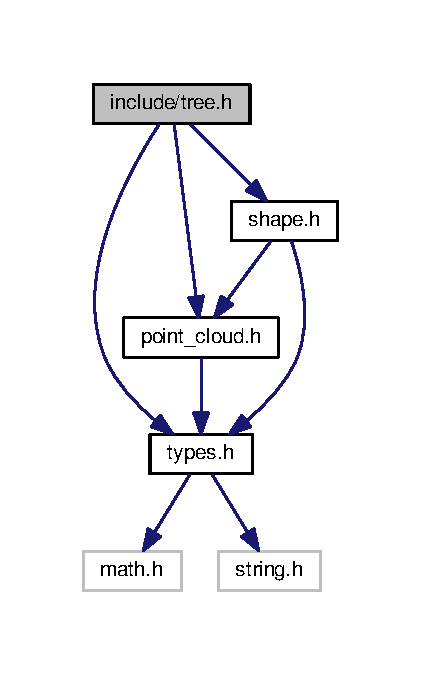
\includegraphics[width=202pt]{tree_8h__incl}
\end{center}
\end{figure}
This graph shows which files directly or indirectly include this file\+:
\nopagebreak
\begin{figure}[H]
\begin{center}
\leavevmode
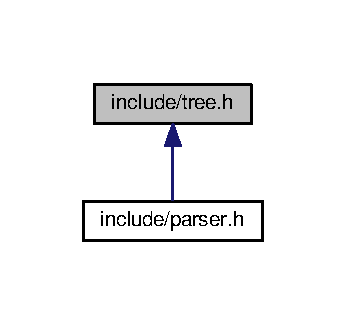
\includegraphics[width=166pt]{tree_8h__dep__incl}
\end{center}
\end{figure}
\subsection*{Data Structures}
\begin{DoxyCompactItemize}
\item 
struct \hyperlink{struct_node}{Node}
\begin{DoxyCompactList}\small\item\em Structure defining a C\+SG tree. \end{DoxyCompactList}\end{DoxyCompactItemize}
\subsection*{Typedefs}
\begin{DoxyCompactItemize}
\item 
typedef struct \hyperlink{struct_node}{Node} $\ast$ \hyperlink{tree_8h_aa8e9e0ac171efcf72384224fafa0915a}{Tree}
\begin{DoxyCompactList}\small\item\em Structure defining a C\+SG tree. \end{DoxyCompactList}\end{DoxyCompactItemize}
\subsection*{Enumerations}
\begin{DoxyCompactItemize}
\item 
enum \hyperlink{tree_8h_a7215803e478cdd4bdf4f1b8087cae87b}{Operator} \{ \\*
\hyperlink{tree_8h_a7215803e478cdd4bdf4f1b8087cae87ba8b8b090d04260fea32aac10ccc01175f}{Union}, 
\hyperlink{tree_8h_a7215803e478cdd4bdf4f1b8087cae87bac852ba2c20196516a8b943442128d21c}{Intersection}, 
\hyperlink{tree_8h_a7215803e478cdd4bdf4f1b8087cae87ba9cba343e00a6259dc83f7e4e7f447109}{Difference}, 
\hyperlink{tree_8h_a7215803e478cdd4bdf4f1b8087cae87ba24f669631df31da9ebff42fc3b49b8df}{Identity}, 
\\*
\hyperlink{tree_8h_a7215803e478cdd4bdf4f1b8087cae87ba7d876d99c658cc26192c3c6804f921e3}{Number\+Operator}
 \}\begin{DoxyCompactList}\small\item\em Enumeration of the different combination operations available. \end{DoxyCompactList}
\end{DoxyCompactItemize}
\subsection*{Functions}
\begin{DoxyCompactItemize}
\item 
\hyperlink{tree_8h_aa8e9e0ac171efcf72384224fafa0915a}{Tree} \hyperlink{tree_8h_aa60547132cb430d5ca8d53193f3b6abd}{tree\+\_\+allocate\+\_\+leaf} (\hyperlink{struct_shape}{Shape} $\ast$shape)
\begin{DoxyCompactList}\small\item\em Allocate a leaf of a C\+SG tree. \end{DoxyCompactList}\item 
\hyperlink{tree_8h_aa8e9e0ac171efcf72384224fafa0915a}{Tree} \hyperlink{tree_8h_a145f24165d53bfdc61f8b5188fa1f3df}{tree\+\_\+allocate\+\_\+node} (\hyperlink{tree_8h_a7215803e478cdd4bdf4f1b8087cae87b}{Operator} op, \hyperlink{tree_8h_aa8e9e0ac171efcf72384224fafa0915a}{Tree} left, \hyperlink{tree_8h_aa8e9e0ac171efcf72384224fafa0915a}{Tree} right)
\begin{DoxyCompactList}\small\item\em Allocate an internal node of a C\+SG tree. \end{DoxyCompactList}\item 
void \hyperlink{tree_8h_a25348c717409522ec53e4f21c0694832}{tree\+\_\+free} (\hyperlink{tree_8h_aa8e9e0ac171efcf72384224fafa0915a}{Tree} $\ast$tree)
\begin{DoxyCompactList}\small\item\em Free the memory allocated by a C\+SG tree. \end{DoxyCompactList}\item 
\hyperlink{struct_point_cloud}{Point\+Cloud} $\ast$ \hyperlink{tree_8h_a83d75ed9c3a3d3ae5c017838c19323b1}{tree\+\_\+to\+\_\+point\+\_\+cloud} (\hyperlink{tree_8h_aa8e9e0ac171efcf72384224fafa0915a}{Tree} tree, int density)
\begin{DoxyCompactList}\small\item\em Convert a C\+SG tree to a point cloud. \end{DoxyCompactList}\item 
void \hyperlink{tree_8h_a41743dcfea9e4f95b025d24b271edb02}{tree\+\_\+homothety} (\hyperlink{tree_8h_aa8e9e0ac171efcf72384224fafa0915a}{Tree} tree, double x, double y, double z)
\begin{DoxyCompactList}\small\item\em Perform an homothety on a C\+SG tree. \end{DoxyCompactList}\item 
int \hyperlink{tree_8h_a964b5db4c8cd5d4ea0e2d019b410a99c}{tree\+\_\+is\+\_\+valid} (\hyperlink{tree_8h_aa8e9e0ac171efcf72384224fafa0915a}{Tree} tree)
\begin{DoxyCompactList}\small\item\em Test if a C\+SG tree datastructure is valid. \end{DoxyCompactList}\item 
void \hyperlink{tree_8h_a06ca6498ae84252b4427a2dc700f15d2}{tree\+\_\+rotation} (\hyperlink{tree_8h_aa8e9e0ac171efcf72384224fafa0915a}{Tree} tree, double x, double y, double z)
\begin{DoxyCompactList}\small\item\em Perform a rotation on a C\+SG tree. \end{DoxyCompactList}\item 
void \hyperlink{tree_8h_a88560e0ec370059ab261331d1a09ea9e}{tree\+\_\+translation} (\hyperlink{tree_8h_aa8e9e0ac171efcf72384224fafa0915a}{Tree} tree, double x, double y, double z)
\begin{DoxyCompactList}\small\item\em Perform a translation on a C\+SG tree. \end{DoxyCompactList}\end{DoxyCompactItemize}


\subsection{Detailed Description}
C\+SG tree management module. 



\subsection{Typedef Documentation}
\index{tree.\+h@{tree.\+h}!Tree@{Tree}}
\index{Tree@{Tree}!tree.\+h@{tree.\+h}}
\subsubsection[{\texorpdfstring{Tree}{Tree}}]{\setlength{\rightskip}{0pt plus 5cm}typedef struct {\bf Node} $\ast$ {\bf Tree}}\hypertarget{tree_8h_aa8e9e0ac171efcf72384224fafa0915a}{}\label{tree_8h_aa8e9e0ac171efcf72384224fafa0915a}


Structure defining a C\+SG tree. 

A C\+SG tree is a recursive structure. If the tree is a leaf, it is defined by a canonical form. If the tree is an internal node, it is defined by a combination operator, a left C\+SG tree child and a right C\+SG tree child. In both cases, the tree also contains a points transformation matrix, an inverse points transformation matrix, and a normals transformation matrix. 

\subsection{Enumeration Type Documentation}
\index{tree.\+h@{tree.\+h}!Operator@{Operator}}
\index{Operator@{Operator}!tree.\+h@{tree.\+h}}
\subsubsection[{\texorpdfstring{Operator}{Operator}}]{\setlength{\rightskip}{0pt plus 5cm}enum {\bf Operator}}\hypertarget{tree_8h_a7215803e478cdd4bdf4f1b8087cae87b}{}\label{tree_8h_a7215803e478cdd4bdf4f1b8087cae87b}


Enumeration of the different combination operations available. 

\begin{Desc}
\item[Enumerator]\par
\begin{description}
\index{Union@{Union}!tree.\+h@{tree.\+h}}\index{tree.\+h@{tree.\+h}!Union@{Union}}\item[{\em 
Union\hypertarget{tree_8h_a7215803e478cdd4bdf4f1b8087cae87ba8b8b090d04260fea32aac10ccc01175f}{}\label{tree_8h_a7215803e478cdd4bdf4f1b8087cae87ba8b8b090d04260fea32aac10ccc01175f}
}]Union (Be careful it is not strictly a mathematical union \+: the intersection is removed) \index{Intersection@{Intersection}!tree.\+h@{tree.\+h}}\index{tree.\+h@{tree.\+h}!Intersection@{Intersection}}\item[{\em 
Intersection\hypertarget{tree_8h_a7215803e478cdd4bdf4f1b8087cae87bac852ba2c20196516a8b943442128d21c}{}\label{tree_8h_a7215803e478cdd4bdf4f1b8087cae87bac852ba2c20196516a8b943442128d21c}
}]Intersection \index{Difference@{Difference}!tree.\+h@{tree.\+h}}\index{tree.\+h@{tree.\+h}!Difference@{Difference}}\item[{\em 
Difference\hypertarget{tree_8h_a7215803e478cdd4bdf4f1b8087cae87ba9cba343e00a6259dc83f7e4e7f447109}{}\label{tree_8h_a7215803e478cdd4bdf4f1b8087cae87ba9cba343e00a6259dc83f7e4e7f447109}
}]Difference \index{Identity@{Identity}!tree.\+h@{tree.\+h}}\index{tree.\+h@{tree.\+h}!Identity@{Identity}}\item[{\em 
Identity\hypertarget{tree_8h_a7215803e478cdd4bdf4f1b8087cae87ba24f669631df31da9ebff42fc3b49b8df}{}\label{tree_8h_a7215803e478cdd4bdf4f1b8087cae87ba24f669631df31da9ebff42fc3b49b8df}
}]Identity (Be careful this operation is a union with intersection kept, be sure then the intersection is empty or it can lead to strange shapes when this operation is composed) \index{Number\+Operator@{Number\+Operator}!tree.\+h@{tree.\+h}}\index{tree.\+h@{tree.\+h}!Number\+Operator@{Number\+Operator}}\item[{\em 
Number\+Operator\hypertarget{tree_8h_a7215803e478cdd4bdf4f1b8087cae87ba7d876d99c658cc26192c3c6804f921e3}{}\label{tree_8h_a7215803e478cdd4bdf4f1b8087cae87ba7d876d99c658cc26192c3c6804f921e3}
}]Number of combination operator \end{description}
\end{Desc}


\subsection{Function Documentation}
\index{tree.\+h@{tree.\+h}!tree\+\_\+allocate\+\_\+leaf@{tree\+\_\+allocate\+\_\+leaf}}
\index{tree\+\_\+allocate\+\_\+leaf@{tree\+\_\+allocate\+\_\+leaf}!tree.\+h@{tree.\+h}}
\subsubsection[{\texorpdfstring{tree\+\_\+allocate\+\_\+leaf(\+Shape $\ast$shape)}{tree_allocate_leaf(Shape *shape)}}]{\setlength{\rightskip}{0pt plus 5cm}{\bf Tree} tree\+\_\+allocate\+\_\+leaf (
\begin{DoxyParamCaption}
\item[{{\bf Shape} $\ast$}]{shape}
\end{DoxyParamCaption}
)}\hypertarget{tree_8h_aa60547132cb430d5ca8d53193f3b6abd}{}\label{tree_8h_aa60547132cb430d5ca8d53193f3b6abd}


Allocate a leaf of a C\+SG tree. 

The program stops if the allocation has failed. This function allocate some memory that need to be freed with {\itshape tree\+\_\+free} 


\begin{DoxyParams}{Parameters}
{\em shape} & Canonical shape ~\newline
Can not take the value {\itshape N\+U\+LL} ~\newline
Must be a valid canonical shape\\
\hline
\end{DoxyParams}
\begin{DoxyReturn}{Returns}
a pointer to the allocated leaf 
\end{DoxyReturn}
\index{tree.\+h@{tree.\+h}!tree\+\_\+allocate\+\_\+node@{tree\+\_\+allocate\+\_\+node}}
\index{tree\+\_\+allocate\+\_\+node@{tree\+\_\+allocate\+\_\+node}!tree.\+h@{tree.\+h}}
\subsubsection[{\texorpdfstring{tree\+\_\+allocate\+\_\+node(\+Operator op, Tree left, Tree right)}{tree_allocate_node(Operator op, Tree left, Tree right)}}]{\setlength{\rightskip}{0pt plus 5cm}{\bf Tree} tree\+\_\+allocate\+\_\+node (
\begin{DoxyParamCaption}
\item[{{\bf Operator}}]{op, }
\item[{{\bf Tree}}]{left, }
\item[{{\bf Tree}}]{right}
\end{DoxyParamCaption}
)}\hypertarget{tree_8h_a145f24165d53bfdc61f8b5188fa1f3df}{}\label{tree_8h_a145f24165d53bfdc61f8b5188fa1f3df}


Allocate an internal node of a C\+SG tree. 

The program stops if the allocation has failed. This function allocate some memory that need to be freed with {\itshape tree\+\_\+free}.


\begin{DoxyParams}{Parameters}
{\em op} & Combination operator at the root of the tree\\
\hline
{\em left} & Left subtree ~\newline
Can not take the value {\itshape N\+U\+LL} ~\newline
Must be a valid C\+SG tree\\
\hline
{\em right} & Right subtree ~\newline
Can not take the value {\itshape N\+U\+LL} ~\newline
Must be a valid C\+SG tree\\
\hline
\end{DoxyParams}
\begin{DoxyReturn}{Returns}
a pointer to the allocated internal node 
\end{DoxyReturn}
\index{tree.\+h@{tree.\+h}!tree\+\_\+free@{tree\+\_\+free}}
\index{tree\+\_\+free@{tree\+\_\+free}!tree.\+h@{tree.\+h}}
\subsubsection[{\texorpdfstring{tree\+\_\+free(\+Tree $\ast$tree)}{tree_free(Tree *tree)}}]{\setlength{\rightskip}{0pt plus 5cm}void tree\+\_\+free (
\begin{DoxyParamCaption}
\item[{{\bf Tree} $\ast$}]{tree}
\end{DoxyParamCaption}
)}\hypertarget{tree_8h_a25348c717409522ec53e4f21c0694832}{}\label{tree_8h_a25348c717409522ec53e4f21c0694832}


Free the memory allocated by a C\+SG tree. 

The pointed C\+SG tree will be set to {\itshape N\+U\+LL}.


\begin{DoxyParams}{Parameters}
{\em shape} & Pointer to the C\+SG tree to free ~\newline
Can not take the value {\itshape N\+U\+LL} ~\newline
Must be a valid C\+SG tree \\
\hline
\end{DoxyParams}
\index{tree.\+h@{tree.\+h}!tree\+\_\+homothety@{tree\+\_\+homothety}}
\index{tree\+\_\+homothety@{tree\+\_\+homothety}!tree.\+h@{tree.\+h}}
\subsubsection[{\texorpdfstring{tree\+\_\+homothety(\+Tree tree, double x, double y, double z)}{tree_homothety(Tree tree, double x, double y, double z)}}]{\setlength{\rightskip}{0pt plus 5cm}void tree\+\_\+homothety (
\begin{DoxyParamCaption}
\item[{{\bf Tree}}]{tree, }
\item[{double}]{x, }
\item[{double}]{y, }
\item[{double}]{z}
\end{DoxyParamCaption}
)}\hypertarget{tree_8h_a41743dcfea9e4f95b025d24b271edb02}{}\label{tree_8h_a41743dcfea9e4f95b025d24b271edb02}


Perform an homothety on a C\+SG tree. 

Operation will update matrix fields of the tree. Scaling factors of canonical shapes at leaves are also updated.


\begin{DoxyParams}{Parameters}
{\em shape} & C\+SG tree to modify ~\newline
Can not take the value {\itshape N\+U\+LL} ~\newline
Must be a valid C\+SG tree\\
\hline
{\em x} & Scaling factor on {\itshape x} axis ~\newline
Must be strictly positive\\
\hline
{\em y} & Scaling factor on {\itshape y} axis ~\newline
Must be strictly positive\\
\hline
{\em z} & Scaling factor on {\itshape z} axis ~\newline
Must be strictly positive \\
\hline
\end{DoxyParams}
\index{tree.\+h@{tree.\+h}!tree\+\_\+is\+\_\+valid@{tree\+\_\+is\+\_\+valid}}
\index{tree\+\_\+is\+\_\+valid@{tree\+\_\+is\+\_\+valid}!tree.\+h@{tree.\+h}}
\subsubsection[{\texorpdfstring{tree\+\_\+is\+\_\+valid(\+Tree tree)}{tree_is_valid(Tree tree)}}]{\setlength{\rightskip}{0pt plus 5cm}int tree\+\_\+is\+\_\+valid (
\begin{DoxyParamCaption}
\item[{{\bf Tree}}]{tree}
\end{DoxyParamCaption}
)}\hypertarget{tree_8h_a964b5db4c8cd5d4ea0e2d019b410a99c}{}\label{tree_8h_a964b5db4c8cd5d4ea0e2d019b410a99c}


Test if a C\+SG tree datastructure is valid. 

A C\+SG tree is valid if \+: ~\newline

\begin{DoxyItemize}
\item {\bfseries tree} is a leaf and {\bfseries shape} is valid ~\newline

\item {\bfseries tree} is internal node and {\bfseries op} is between {\itshape 0} and {\itshape Number\+Operator-\/1} ~\newline

\item {\bfseries tree} is internal node and {\bfseries left} is different from {\itshape N\+U\+LL} ~\newline

\item {\bfseries tree} is internal node and {\bfseries right} is different from {\itshape N\+U\+LL} 
\end{DoxyItemize}


\begin{DoxyParams}{Parameters}
{\em tree} & C\+SG tree to test ~\newline
Can not take the value {\itshape N\+U\+LL} ~\newline
 \\
\hline
\end{DoxyParams}
\begin{DoxyReturn}{Returns}
{\itshape 1} if C\+SG tree is valid, {\itshape 0} otherwise 
\end{DoxyReturn}
\index{tree.\+h@{tree.\+h}!tree\+\_\+rotation@{tree\+\_\+rotation}}
\index{tree\+\_\+rotation@{tree\+\_\+rotation}!tree.\+h@{tree.\+h}}
\subsubsection[{\texorpdfstring{tree\+\_\+rotation(\+Tree tree, double x, double y, double z)}{tree_rotation(Tree tree, double x, double y, double z)}}]{\setlength{\rightskip}{0pt plus 5cm}void tree\+\_\+rotation (
\begin{DoxyParamCaption}
\item[{{\bf Tree}}]{tree, }
\item[{double}]{x, }
\item[{double}]{y, }
\item[{double}]{z}
\end{DoxyParamCaption}
)}\hypertarget{tree_8h_a06ca6498ae84252b4427a2dc700f15d2}{}\label{tree_8h_a06ca6498ae84252b4427a2dc700f15d2}


Perform a rotation on a C\+SG tree. 

Operation will update matrix fields of the tree.


\begin{DoxyParams}{Parameters}
{\em shape} & C\+SG tree to modify ~\newline
Can not take the value {\itshape N\+U\+LL} ~\newline
Must be a valid C\+SG tree\\
\hline
{\em x} & Rotation angle around {\itshape x} axis\\
\hline
{\em y} & Rotation angle around {\itshape y} axis\\
\hline
{\em z} & Rotation angle around {\itshape z} axis \\
\hline
\end{DoxyParams}
\index{tree.\+h@{tree.\+h}!tree\+\_\+to\+\_\+point\+\_\+cloud@{tree\+\_\+to\+\_\+point\+\_\+cloud}}
\index{tree\+\_\+to\+\_\+point\+\_\+cloud@{tree\+\_\+to\+\_\+point\+\_\+cloud}!tree.\+h@{tree.\+h}}
\subsubsection[{\texorpdfstring{tree\+\_\+to\+\_\+point\+\_\+cloud(\+Tree tree, int density)}{tree_to_point_cloud(Tree tree, int density)}}]{\setlength{\rightskip}{0pt plus 5cm}{\bf Point\+Cloud}$\ast$ tree\+\_\+to\+\_\+point\+\_\+cloud (
\begin{DoxyParamCaption}
\item[{{\bf Tree}}]{tree, }
\item[{int}]{density}
\end{DoxyParamCaption}
)}\hypertarget{tree_8h_a83d75ed9c3a3d3ae5c017838c19323b1}{}\label{tree_8h_a83d75ed9c3a3d3ae5c017838c19323b1}


Convert a C\+SG tree to a point cloud. 

This function is necessary in order to be able to the render a C\+SG tree. This function allocate some memory that need to be freed with {\itshape point\+\_\+cloud\+\_\+free}.


\begin{DoxyParams}{Parameters}
{\em shape} & C\+SG tree to convert ~\newline
Can not take the value {\itshape N\+U\+LL} ~\newline
Must be a valid C\+SG tree\\
\hline
{\em density} & Point density per unit area ~\newline
Must be strictly positive\\
\hline
\end{DoxyParams}
\begin{DoxyReturn}{Returns}
a pointer to the allocated point cloud 
\end{DoxyReturn}
\index{tree.\+h@{tree.\+h}!tree\+\_\+translation@{tree\+\_\+translation}}
\index{tree\+\_\+translation@{tree\+\_\+translation}!tree.\+h@{tree.\+h}}
\subsubsection[{\texorpdfstring{tree\+\_\+translation(\+Tree tree, double x, double y, double z)}{tree_translation(Tree tree, double x, double y, double z)}}]{\setlength{\rightskip}{0pt plus 5cm}void tree\+\_\+translation (
\begin{DoxyParamCaption}
\item[{{\bf Tree}}]{tree, }
\item[{double}]{x, }
\item[{double}]{y, }
\item[{double}]{z}
\end{DoxyParamCaption}
)}\hypertarget{tree_8h_a88560e0ec370059ab261331d1a09ea9e}{}\label{tree_8h_a88560e0ec370059ab261331d1a09ea9e}


Perform a translation on a C\+SG tree. 

Operation will update matrix fields of the tree.


\begin{DoxyParams}{Parameters}
{\em shape} & C\+SG tree to modify ~\newline
Can not take the value {\itshape N\+U\+LL} ~\newline
Must be a valid C\+SG tree\\
\hline
{\em x} & Translation factor on {\itshape x} axis\\
\hline
{\em y} & Translation factor on {\itshape y} axis\\
\hline
{\em z} & Translation factor on {\itshape z} axis \\
\hline
\end{DoxyParams}

\hypertarget{types_8h}{}\section{include/types.h File Reference}
\label{types_8h}\index{include/types.\+h@{include/types.\+h}}


basic operations management module  


{\ttfamily \#include $<$math.\+h$>$}\\*
{\ttfamily \#include $<$string.\+h$>$}\\*
Include dependency graph for types.\+h\+:
\nopagebreak
\begin{figure}[H]
\begin{center}
\leavevmode
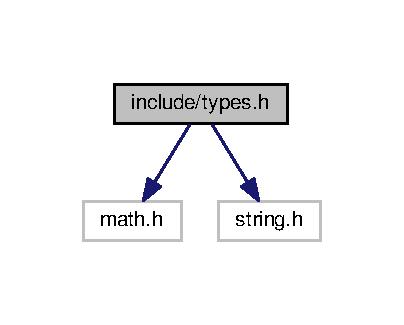
\includegraphics[width=194pt]{types_8h__incl}
\end{center}
\end{figure}
This graph shows which files directly or indirectly include this file\+:
\nopagebreak
\begin{figure}[H]
\begin{center}
\leavevmode
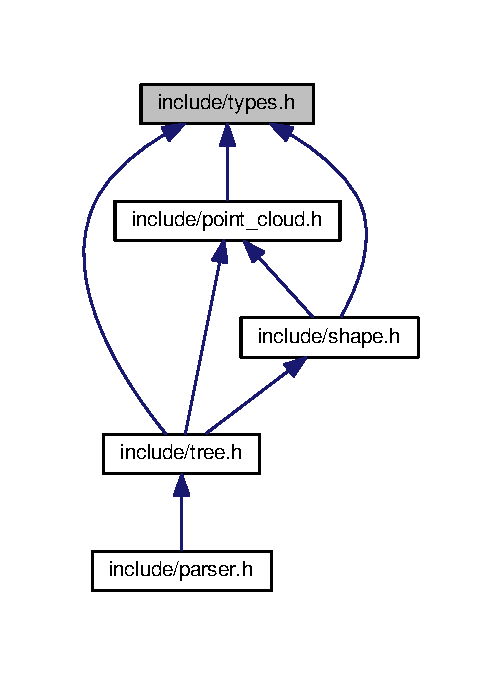
\includegraphics[width=241pt]{types_8h__dep__incl}
\end{center}
\end{figure}
\subsection*{Macros}
\begin{DoxyCompactItemize}
\item 
\#define \hyperlink{types_8h_a598a3330b3c21701223ee0ca14316eca}{PI}~3.\+1415926535897932384626433832795\hypertarget{types_8h_a598a3330b3c21701223ee0ca14316eca}{}\label{types_8h_a598a3330b3c21701223ee0ca14316eca}

\begin{DoxyCompactList}\small\item\em Value of pi. \end{DoxyCompactList}\item 
\#define \hyperlink{types_8h_adc79c67a861395580961f87d80f38483}{S\+Q\+U\+A\+RE}(a)~((a)$\ast$(a))\hypertarget{types_8h_adc79c67a861395580961f87d80f38483}{}\label{types_8h_adc79c67a861395580961f87d80f38483}

\begin{DoxyCompactList}\small\item\em Macro to compute square value. \end{DoxyCompactList}\item 
\#define \hyperlink{types_8h_a4887ceeae88266064841cbbc11ef8b53}{M\+I\+N3}(a,  b,  c)~(((a)$<$(b))?(((a)$<$(c))?(a)\+:(c))\+:(((b)$<$(c))?(b)\+:(c)))\hypertarget{types_8h_a4887ceeae88266064841cbbc11ef8b53}{}\label{types_8h_a4887ceeae88266064841cbbc11ef8b53}

\begin{DoxyCompactList}\small\item\em Macro to compute the minimum of 3 numbers. \end{DoxyCompactList}\item 
\#define \hyperlink{types_8h_a37c6d7fcb9c177c308ef38e1d51d35e3}{M\+A\+X3}(a,  b,  c)~(((a)$>$(b))?(((a)$>$(c))?(a)\+:(c))\+:(((b)$>$(c))?(b)\+:(c)))\hypertarget{types_8h_a37c6d7fcb9c177c308ef38e1d51d35e3}{}\label{types_8h_a37c6d7fcb9c177c308ef38e1d51d35e3}

\begin{DoxyCompactList}\small\item\em Macro to compute the maximum of 3 numbers. \end{DoxyCompactList}\item 
\#define \hyperlink{types_8h_aceb8d2eb1bd7b0cc483838df3950a6c2}{color4\+\_\+set}(color,  r,  g,  b,  a)
\begin{DoxyCompactList}\small\item\em Set the values of a color. \end{DoxyCompactList}\item 
\#define \hyperlink{types_8h_a424599ea02cabdb5652b4874b2b662c3}{color4\+\_\+copy}(color1,  color2)
\begin{DoxyCompactList}\small\item\em Copy a color. \end{DoxyCompactList}\item 
\#define \hyperlink{types_8h_a325390279657de3053b53634d0121058}{color4\+\_\+scale}(color,  s)
\begin{DoxyCompactList}\small\item\em Scale a color. \end{DoxyCompactList}\item 
\#define \hyperlink{types_8h_a0e6507d156017a87d6e28b776ea163bd}{coord3\+\_\+get\+\_\+x}(c)~((c)\mbox{[}0\mbox{]})
\begin{DoxyCompactList}\small\item\em Get the {\itshape x} value of the coordinate. \end{DoxyCompactList}\item 
\#define \hyperlink{types_8h_aa2df190eca61e8a453cf5d0693194561}{coord3\+\_\+get\+\_\+y}(c)~((c)\mbox{[}1\mbox{]})
\begin{DoxyCompactList}\small\item\em Get the {\itshape y} value of the coordinate. \end{DoxyCompactList}\item 
\#define \hyperlink{types_8h_ace10a3a665f571c0c3b392c1d18ec793}{coord3\+\_\+get\+\_\+z}(c)~((c)\mbox{[}2\mbox{]})
\begin{DoxyCompactList}\small\item\em Get the {\itshape z} value of the coordinate. \end{DoxyCompactList}\item 
\#define \hyperlink{types_8h_a81f2675fdce2bd8c7f12d794f9026f7d}{coord3\+\_\+set}(c,  x,  y,  z)
\begin{DoxyCompactList}\small\item\em Set the values of a coordinate. \end{DoxyCompactList}\item 
\#define \hyperlink{types_8h_a5c1dbd92d1b9987c966a1375be7103d7}{coord3\+\_\+copy}(c1,  c2)
\begin{DoxyCompactList}\small\item\em Copy a coordinate. \end{DoxyCompactList}\item 
\#define \hyperlink{types_8h_a734a94bc6b27d684511f599add38db54}{coord3\+\_\+scale}(c,  s)
\begin{DoxyCompactList}\small\item\em Scale a coordinate. \end{DoxyCompactList}\item 
\#define \hyperlink{types_8h_a4b91fdc5bc65c41a9200e0899ac3b9ac}{point3\+\_\+get\+\_\+x}(p)~(\hyperlink{types_8h_a0e6507d156017a87d6e28b776ea163bd}{coord3\+\_\+get\+\_\+x}(p))
\begin{DoxyCompactList}\small\item\em Get the {\itshape x} value of the point. \end{DoxyCompactList}\item 
\#define \hyperlink{types_8h_a7fd5ddbe671c68fd2db9a305cda24f03}{point3\+\_\+get\+\_\+y}(p)~(\hyperlink{types_8h_aa2df190eca61e8a453cf5d0693194561}{coord3\+\_\+get\+\_\+y}(p))
\begin{DoxyCompactList}\small\item\em Get the {\itshape y} value of the point. \end{DoxyCompactList}\item 
\#define \hyperlink{types_8h_aab9c252b6500d561b325a730b07f5c52}{point3\+\_\+get\+\_\+z}(p)~(\hyperlink{types_8h_ace10a3a665f571c0c3b392c1d18ec793}{coord3\+\_\+get\+\_\+z}(p))
\begin{DoxyCompactList}\small\item\em Get the {\itshape z} value of the point. \end{DoxyCompactList}\item 
\#define \hyperlink{types_8h_a00c22f58e83df581b700ab32475be0dc}{point3\+\_\+copy}(p1,  p2)~(\hyperlink{types_8h_a5c1dbd92d1b9987c966a1375be7103d7}{coord3\+\_\+copy}(p1, p2))
\begin{DoxyCompactList}\small\item\em Copy a point. \end{DoxyCompactList}\item 
\#define \hyperlink{types_8h_a462c456993f95e164724f36276741b87}{point3\+\_\+set}(p,  x,  y,  z)~(\hyperlink{types_8h_a81f2675fdce2bd8c7f12d794f9026f7d}{coord3\+\_\+set}(p, x, y, z))
\begin{DoxyCompactList}\small\item\em Set the values of a point. \end{DoxyCompactList}\item 
\#define \hyperlink{types_8h_a3136eab3453fdb656783f4690ef6adf7}{point3\+\_\+from\+\_\+to\+\_\+vector}(p1,  p2)
\begin{DoxyCompactList}\small\item\em Compute the vector between two points. \end{DoxyCompactList}\item 
\#define \hyperlink{types_8h_a2a924158373bde7181e6b522a11aef6a}{vec3\+\_\+get\+\_\+x}(v)~(\hyperlink{types_8h_a0e6507d156017a87d6e28b776ea163bd}{coord3\+\_\+get\+\_\+x}(v))
\begin{DoxyCompactList}\small\item\em Get the {\itshape x} value of the vector. \end{DoxyCompactList}\item 
\#define \hyperlink{types_8h_a003ad5286beb42db2625e0b4fd72407f}{vec3\+\_\+get\+\_\+y}(v)~(\hyperlink{types_8h_aa2df190eca61e8a453cf5d0693194561}{coord3\+\_\+get\+\_\+y}(v))
\begin{DoxyCompactList}\small\item\em Get the {\itshape y} value of the vector. \end{DoxyCompactList}\item 
\#define \hyperlink{types_8h_ac31f9c62ed1557eef70c2b5c8e6283ba}{vec3\+\_\+get\+\_\+z}(v)~(\hyperlink{types_8h_ace10a3a665f571c0c3b392c1d18ec793}{coord3\+\_\+get\+\_\+z}(v))
\begin{DoxyCompactList}\small\item\em Get the {\itshape z} value of the vector. \end{DoxyCompactList}\item 
\#define \hyperlink{types_8h_a2758d5b0fcab1709d6a91e516d065fcb}{vec3\+\_\+copy}(v1,  v2)~(\hyperlink{types_8h_a5c1dbd92d1b9987c966a1375be7103d7}{coord3\+\_\+copy}(v1, v2))
\begin{DoxyCompactList}\small\item\em Copy a vector. \end{DoxyCompactList}\item 
\#define \hyperlink{types_8h_ab0927a15b4cf77b9f8234ac9004cbe13}{vec3\+\_\+set}(v,  x,  y,  z)~(\hyperlink{types_8h_a81f2675fdce2bd8c7f12d794f9026f7d}{coord3\+\_\+set}(v, x, y, z))
\begin{DoxyCompactList}\small\item\em Set the values of a vector. \end{DoxyCompactList}\item 
\#define \hyperlink{types_8h_aef59c6d3dda785a9de5fccdefc735f94}{vec3\+\_\+scale}(v,  s)~(\hyperlink{types_8h_a734a94bc6b27d684511f599add38db54}{coord3\+\_\+scale}(v, s))
\begin{DoxyCompactList}\small\item\em Scale a vector. \end{DoxyCompactList}\item 
\#define \hyperlink{types_8h_a5123adaf5166cd1e8c6b1a160ffb4293}{vec3\+\_\+dot}(u,  v)~((u)\mbox{[}0\mbox{]}$\ast$(v)\mbox{[}0\mbox{]}+(u)\mbox{[}1\mbox{]}$\ast$(v)\mbox{[}1\mbox{]}+(u)\mbox{[}2\mbox{]}$\ast$(v)\mbox{[}2\mbox{]})
\begin{DoxyCompactList}\small\item\em Compute the dot product of vectors. \end{DoxyCompactList}\item 
\#define \hyperlink{types_8h_a1d194846f861cd9ac4cc54ec7032521a}{vec3\+\_\+cross}(result,  u,  v)
\begin{DoxyCompactList}\small\item\em Compute the cross product of vectors. \end{DoxyCompactList}\item 
\#define \hyperlink{types_8h_ad1ecfbb39f5318b6865b588d0f1c610b}{vec3\+\_\+norm}(v)~(sqrt(\hyperlink{types_8h_a5123adaf5166cd1e8c6b1a160ffb4293}{vec3\+\_\+dot}(v,v)))
\begin{DoxyCompactList}\small\item\em Compute the norm of the vector. \end{DoxyCompactList}\item 
\#define \hyperlink{types_8h_ac15cab5e60c70b5263110828da31896d}{mat4\+\_\+set}(m,  col,  line,  val)~((m)\mbox{[}4$\ast$(col)+(line)\mbox{]}=(val))
\begin{DoxyCompactList}\small\item\em Set a value in the homogeneous matrix. \end{DoxyCompactList}\item 
\#define \hyperlink{types_8h_a41c1afaf8c5241ce7d09fe88968202ce}{mat4\+\_\+get}(m,  col,  line)~((m)\mbox{[}4$\ast$(col)+(line)\mbox{]})
\begin{DoxyCompactList}\small\item\em Get a value in the homogeneous matrix. \end{DoxyCompactList}\item 
\#define \hyperlink{types_8h_ae494ebe1b149e5915fbc619b879ddaab}{mat4\+\_\+identity}
\begin{DoxyCompactList}\small\item\em The indentiy homogeneous matrix. \end{DoxyCompactList}\item 
\#define \hyperlink{types_8h_a5f4474fefdd6ab87abd602ceeac262eb}{mat4\+\_\+set\+\_\+identity}(m)
\begin{DoxyCompactList}\small\item\em Set the identity matrix in the homogeneous matrix. \end{DoxyCompactList}\end{DoxyCompactItemize}
\subsection*{Typedefs}
\begin{DoxyCompactItemize}
\item 
typedef float \hyperlink{types_8h_a3d75ae93fc87c7ef6399af18de18ed4a}{color4}\mbox{[}4\mbox{]}
\begin{DoxyCompactList}\small\item\em Structure defining a color. \end{DoxyCompactList}\item 
typedef double \hyperlink{types_8h_a5f1e5af91b8468422981c7f1fa9c6b72}{coord3}\mbox{[}3\mbox{]}
\begin{DoxyCompactList}\small\item\em Structure defining a 3D coordinate. \end{DoxyCompactList}\item 
typedef \hyperlink{types_8h_a5f1e5af91b8468422981c7f1fa9c6b72}{coord3} \hyperlink{types_8h_a5680245085eb6c3661c1ec194979ccd2}{point3}
\begin{DoxyCompactList}\small\item\em Structure defining a 3D point. \end{DoxyCompactList}\item 
typedef \hyperlink{types_8h_a5f1e5af91b8468422981c7f1fa9c6b72}{coord3} \hyperlink{types_8h_a1c0f6462cae9caa5b9f49d5ffd32af60}{vec3}
\begin{DoxyCompactList}\small\item\em Structure defining a 3D vector. \end{DoxyCompactList}\item 
typedef double \hyperlink{types_8h_af8defaae7643cbe46b09ad8dea2eca9b}{mat4}\mbox{[}16\mbox{]}
\begin{DoxyCompactList}\small\item\em Structure defining a 3D homogeneous matrix. \end{DoxyCompactList}\end{DoxyCompactItemize}
\subsection*{Functions}
\begin{DoxyCompactItemize}
\item 
void \hyperlink{types_8h_ad841d2a1d1bbb9b5db0714873ae9403c}{vec3\+\_\+normalize} (\hyperlink{types_8h_a1c0f6462cae9caa5b9f49d5ffd32af60}{vec3} v)
\begin{DoxyCompactList}\small\item\em Compute a product between a homogeneous matrix and a point. \end{DoxyCompactList}\item 
void \hyperlink{types_8h_a7128234a520c6508abc09872e280175b}{mat4\+\_\+translation} (\hyperlink{types_8h_af8defaae7643cbe46b09ad8dea2eca9b}{mat4} m, double tx, double ty, double tz)
\begin{DoxyCompactList}\small\item\em Compute a translation matrix. \end{DoxyCompactList}\item 
void \hyperlink{types_8h_a4cbb4e49491fbbd534c0dcb6e7e7f7e5}{mat4\+\_\+homothety} (\hyperlink{types_8h_af8defaae7643cbe46b09ad8dea2eca9b}{mat4} m, double hx, double hy, double hz)
\begin{DoxyCompactList}\small\item\em Compute a homothety matrix. \end{DoxyCompactList}\item 
void \hyperlink{types_8h_a587f38fa8f5678c880de6c9c6be6b961}{mat4\+\_\+rotation\+\_\+x} (\hyperlink{types_8h_af8defaae7643cbe46b09ad8dea2eca9b}{mat4} m, double alpha)
\begin{DoxyCompactList}\small\item\em Compute a rotation matrix around x axis. \end{DoxyCompactList}\item 
void \hyperlink{types_8h_a701aa0608f011dbe678ef2bc47027ace}{mat4\+\_\+rotation\+\_\+y} (\hyperlink{types_8h_af8defaae7643cbe46b09ad8dea2eca9b}{mat4} m, double alpha)
\begin{DoxyCompactList}\small\item\em Compute a rotation matrix around y axis. \end{DoxyCompactList}\item 
void \hyperlink{types_8h_acb138034ba4797bfdd0b4ae27407af43}{mat4\+\_\+rotation\+\_\+z} (\hyperlink{types_8h_af8defaae7643cbe46b09ad8dea2eca9b}{mat4} m, double alpha)
\begin{DoxyCompactList}\small\item\em Compute a rotation matrix around z axis. \end{DoxyCompactList}\item 
void \hyperlink{types_8h_af07c7e092abda85a8c827557225ff99c}{mat4\+\_\+product\+\_\+mat4} (\hyperlink{types_8h_af8defaae7643cbe46b09ad8dea2eca9b}{mat4} m\+\_\+result, \hyperlink{types_8h_af8defaae7643cbe46b09ad8dea2eca9b}{mat4} m1, \hyperlink{types_8h_af8defaae7643cbe46b09ad8dea2eca9b}{mat4} m2)
\begin{DoxyCompactList}\small\item\em Compute a product between homogeneous matrices. \end{DoxyCompactList}\item 
void \hyperlink{types_8h_ad20035b6b8a9f3aa2dbb128ae5d8904a}{mat4\+\_\+product\+\_\+vec3} (\hyperlink{types_8h_a1c0f6462cae9caa5b9f49d5ffd32af60}{vec3} v\+\_\+result, \hyperlink{types_8h_af8defaae7643cbe46b09ad8dea2eca9b}{mat4} m, \hyperlink{types_8h_a1c0f6462cae9caa5b9f49d5ffd32af60}{vec3} v)
\begin{DoxyCompactList}\small\item\em Compute a product between a homogeneous matrix and a vector. \end{DoxyCompactList}\item 
void \hyperlink{types_8h_a29167f1e556ed3bfb7cbc24fef89690a}{mat4\+\_\+product\+\_\+point3} (\hyperlink{types_8h_a5680245085eb6c3661c1ec194979ccd2}{point3} p\+\_\+result, \hyperlink{types_8h_af8defaae7643cbe46b09ad8dea2eca9b}{mat4} m, \hyperlink{types_8h_a5680245085eb6c3661c1ec194979ccd2}{point3} p)
\begin{DoxyCompactList}\small\item\em Compute a product between a homogeneous matrix and a point. \end{DoxyCompactList}\end{DoxyCompactItemize}


\subsection{Detailed Description}
basic operations management module 



\subsection{Macro Definition Documentation}
\index{types.\+h@{types.\+h}!color4\+\_\+copy@{color4\+\_\+copy}}
\index{color4\+\_\+copy@{color4\+\_\+copy}!types.\+h@{types.\+h}}
\subsubsection[{\texorpdfstring{color4\+\_\+copy}{color4_copy}}]{\setlength{\rightskip}{0pt plus 5cm}\#define color4\+\_\+copy(
\begin{DoxyParamCaption}
\item[{}]{color1, }
\item[{}]{color2}
\end{DoxyParamCaption}
)}\hypertarget{types_8h_a424599ea02cabdb5652b4874b2b662c3}{}\label{types_8h_a424599ea02cabdb5652b4874b2b662c3}
{\bfseries Value\+:}
\begin{DoxyCode}
((color1)[0]=(color2)[0],\(\backslash\)
                                     (color1)[1]=(color2)[1],\(\backslash\)
                                     (color1)[2]=(color2)[2],\(\backslash\)
                                     (color1)[3]=(color2)[3])
\end{DoxyCode}


Copy a color. 


\begin{DoxyParams}{Parameters}
{\em color1} & Color to modify\\
\hline
{\em color2} & Color to copy \\
\hline
\end{DoxyParams}
\index{types.\+h@{types.\+h}!color4\+\_\+scale@{color4\+\_\+scale}}
\index{color4\+\_\+scale@{color4\+\_\+scale}!types.\+h@{types.\+h}}
\subsubsection[{\texorpdfstring{color4\+\_\+scale}{color4_scale}}]{\setlength{\rightskip}{0pt plus 5cm}\#define color4\+\_\+scale(
\begin{DoxyParamCaption}
\item[{}]{color, }
\item[{}]{s}
\end{DoxyParamCaption}
)}\hypertarget{types_8h_a325390279657de3053b53634d0121058}{}\label{types_8h_a325390279657de3053b53634d0121058}
{\bfseries Value\+:}
\begin{DoxyCode}
\{(color)[0]*s,\(\backslash\)
                               (color)[1]*s,\(\backslash\)
                               (color)[2]*s,\(\backslash\)
                               (color)[3]*s\}
\end{DoxyCode}


Scale a color. 


\begin{DoxyParams}{Parameters}
{\em color} & Color to modify\\
\hline
{\em s} & Scaling factor\\
\hline
\end{DoxyParams}
\begin{DoxyReturn}{Returns}
a scaled color 
\end{DoxyReturn}
\index{types.\+h@{types.\+h}!color4\+\_\+set@{color4\+\_\+set}}
\index{color4\+\_\+set@{color4\+\_\+set}!types.\+h@{types.\+h}}
\subsubsection[{\texorpdfstring{color4\+\_\+set}{color4_set}}]{\setlength{\rightskip}{0pt plus 5cm}\#define color4\+\_\+set(
\begin{DoxyParamCaption}
\item[{}]{color, }
\item[{}]{r, }
\item[{}]{g, }
\item[{}]{b, }
\item[{}]{a}
\end{DoxyParamCaption}
)}\hypertarget{types_8h_aceb8d2eb1bd7b0cc483838df3950a6c2}{}\label{types_8h_aceb8d2eb1bd7b0cc483838df3950a6c2}
{\bfseries Value\+:}
\begin{DoxyCode}
((color)[0]=(r),\(\backslash\)
                                   (color)[1]=(g),\(\backslash\)
                                   (color)[2]=(b),\(\backslash\)
                                   (color)[3]=(a))
\end{DoxyCode}


Set the values of a color. 


\begin{DoxyParams}{Parameters}
{\em color} & Color to modify\\
\hline
{\em r} & Red value of color\\
\hline
{\em r} & Green value of color\\
\hline
{\em r} & Blue value of color\\
\hline
{\em a} & Alpha value of color \\
\hline
\end{DoxyParams}
\index{types.\+h@{types.\+h}!coord3\+\_\+copy@{coord3\+\_\+copy}}
\index{coord3\+\_\+copy@{coord3\+\_\+copy}!types.\+h@{types.\+h}}
\subsubsection[{\texorpdfstring{coord3\+\_\+copy}{coord3_copy}}]{\setlength{\rightskip}{0pt plus 5cm}\#define coord3\+\_\+copy(
\begin{DoxyParamCaption}
\item[{}]{c1, }
\item[{}]{c2}
\end{DoxyParamCaption}
)}\hypertarget{types_8h_a5c1dbd92d1b9987c966a1375be7103d7}{}\label{types_8h_a5c1dbd92d1b9987c966a1375be7103d7}
{\bfseries Value\+:}
\begin{DoxyCode}
((c1)[0]=(c2)[0],\(\backslash\)
                             (c1)[1]=(c2)[1],\(\backslash\)
                             (c1)[2]=(c2)[2])
\end{DoxyCode}


Copy a coordinate. 


\begin{DoxyParams}{Parameters}
{\em c1} & Coordinate to modify\\
\hline
{\em c2} & Coordinate to copy \\
\hline
\end{DoxyParams}
\index{types.\+h@{types.\+h}!coord3\+\_\+get\+\_\+x@{coord3\+\_\+get\+\_\+x}}
\index{coord3\+\_\+get\+\_\+x@{coord3\+\_\+get\+\_\+x}!types.\+h@{types.\+h}}
\subsubsection[{\texorpdfstring{coord3\+\_\+get\+\_\+x}{coord3_get_x}}]{\setlength{\rightskip}{0pt plus 5cm}\#define coord3\+\_\+get\+\_\+x(
\begin{DoxyParamCaption}
\item[{}]{c}
\end{DoxyParamCaption}
)~((c)\mbox{[}0\mbox{]})}\hypertarget{types_8h_a0e6507d156017a87d6e28b776ea163bd}{}\label{types_8h_a0e6507d156017a87d6e28b776ea163bd}


Get the {\itshape x} value of the coordinate. 


\begin{DoxyParams}{Parameters}
{\em c} & Coordinate\\
\hline
\end{DoxyParams}
\begin{DoxyReturn}{Returns}
the {\itshape x} value of the coordinate 
\end{DoxyReturn}
\index{types.\+h@{types.\+h}!coord3\+\_\+get\+\_\+y@{coord3\+\_\+get\+\_\+y}}
\index{coord3\+\_\+get\+\_\+y@{coord3\+\_\+get\+\_\+y}!types.\+h@{types.\+h}}
\subsubsection[{\texorpdfstring{coord3\+\_\+get\+\_\+y}{coord3_get_y}}]{\setlength{\rightskip}{0pt plus 5cm}\#define coord3\+\_\+get\+\_\+y(
\begin{DoxyParamCaption}
\item[{}]{c}
\end{DoxyParamCaption}
)~((c)\mbox{[}1\mbox{]})}\hypertarget{types_8h_aa2df190eca61e8a453cf5d0693194561}{}\label{types_8h_aa2df190eca61e8a453cf5d0693194561}


Get the {\itshape y} value of the coordinate. 


\begin{DoxyParams}{Parameters}
{\em c} & Coordinate\\
\hline
\end{DoxyParams}
\begin{DoxyReturn}{Returns}
the {\itshape y} value of the coordinate 
\end{DoxyReturn}
\index{types.\+h@{types.\+h}!coord3\+\_\+get\+\_\+z@{coord3\+\_\+get\+\_\+z}}
\index{coord3\+\_\+get\+\_\+z@{coord3\+\_\+get\+\_\+z}!types.\+h@{types.\+h}}
\subsubsection[{\texorpdfstring{coord3\+\_\+get\+\_\+z}{coord3_get_z}}]{\setlength{\rightskip}{0pt plus 5cm}\#define coord3\+\_\+get\+\_\+z(
\begin{DoxyParamCaption}
\item[{}]{c}
\end{DoxyParamCaption}
)~((c)\mbox{[}2\mbox{]})}\hypertarget{types_8h_ace10a3a665f571c0c3b392c1d18ec793}{}\label{types_8h_ace10a3a665f571c0c3b392c1d18ec793}


Get the {\itshape z} value of the coordinate. 


\begin{DoxyParams}{Parameters}
{\em c} & Coordinate\\
\hline
\end{DoxyParams}
\begin{DoxyReturn}{Returns}
the {\itshape z} value of the coordinate 
\end{DoxyReturn}
\index{types.\+h@{types.\+h}!coord3\+\_\+scale@{coord3\+\_\+scale}}
\index{coord3\+\_\+scale@{coord3\+\_\+scale}!types.\+h@{types.\+h}}
\subsubsection[{\texorpdfstring{coord3\+\_\+scale}{coord3_scale}}]{\setlength{\rightskip}{0pt plus 5cm}\#define coord3\+\_\+scale(
\begin{DoxyParamCaption}
\item[{}]{c, }
\item[{}]{s}
\end{DoxyParamCaption}
)}\hypertarget{types_8h_a734a94bc6b27d684511f599add38db54}{}\label{types_8h_a734a94bc6b27d684511f599add38db54}
{\bfseries Value\+:}
\begin{DoxyCode}
\{(c)[0]*s,\(\backslash\)
                            (c)[1]*s,\(\backslash\)
                            (c)[2]*s\}
\end{DoxyCode}


Scale a coordinate. 


\begin{DoxyParams}{Parameters}
{\em color} & Coordinate to modify\\
\hline
{\em s} & Scaling factor\\
\hline
\end{DoxyParams}
\begin{DoxyReturn}{Returns}
a scaled coordinate 
\end{DoxyReturn}
\index{types.\+h@{types.\+h}!coord3\+\_\+set@{coord3\+\_\+set}}
\index{coord3\+\_\+set@{coord3\+\_\+set}!types.\+h@{types.\+h}}
\subsubsection[{\texorpdfstring{coord3\+\_\+set}{coord3_set}}]{\setlength{\rightskip}{0pt plus 5cm}\#define coord3\+\_\+set(
\begin{DoxyParamCaption}
\item[{}]{c, }
\item[{}]{x, }
\item[{}]{y, }
\item[{}]{z}
\end{DoxyParamCaption}
)}\hypertarget{types_8h_a81f2675fdce2bd8c7f12d794f9026f7d}{}\label{types_8h_a81f2675fdce2bd8c7f12d794f9026f7d}
{\bfseries Value\+:}
\begin{DoxyCode}
((c)[0]=(x),\(\backslash\)
                                (c)[1]=(y),\(\backslash\)
                                (c)[2]=(z))
\end{DoxyCode}


Set the values of a coordinate. 


\begin{DoxyParams}{Parameters}
{\em v} & Coordinate to modify\\
\hline
{\em x} & Value of the coordinate on {\itshape x} axis\\
\hline
{\em y} & Value of the coordinate on {\itshape y} axis\\
\hline
{\em z} & Value of the coordinate on {\itshape z} axis \\
\hline
\end{DoxyParams}
\index{types.\+h@{types.\+h}!mat4\+\_\+get@{mat4\+\_\+get}}
\index{mat4\+\_\+get@{mat4\+\_\+get}!types.\+h@{types.\+h}}
\subsubsection[{\texorpdfstring{mat4\+\_\+get}{mat4_get}}]{\setlength{\rightskip}{0pt plus 5cm}\#define mat4\+\_\+get(
\begin{DoxyParamCaption}
\item[{}]{m, }
\item[{}]{col, }
\item[{}]{line}
\end{DoxyParamCaption}
)~((m)\mbox{[}4$\ast$(col)+(line)\mbox{]})}\hypertarget{types_8h_a41c1afaf8c5241ce7d09fe88968202ce}{}\label{types_8h_a41c1afaf8c5241ce7d09fe88968202ce}


Get a value in the homogeneous matrix. 


\begin{DoxyParams}{Parameters}
{\em m} & Homogeneous matrix\\
\hline
{\em col} & Column index\\
\hline
{\em col} & Line index\\
\hline
\end{DoxyParams}
\begin{DoxyReturn}{Returns}
value of the homogeneous matrix at given indices 
\end{DoxyReturn}
\index{types.\+h@{types.\+h}!mat4\+\_\+identity@{mat4\+\_\+identity}}
\index{mat4\+\_\+identity@{mat4\+\_\+identity}!types.\+h@{types.\+h}}
\subsubsection[{\texorpdfstring{mat4\+\_\+identity}{mat4_identity}}]{\setlength{\rightskip}{0pt plus 5cm}\#define mat4\+\_\+identity}\hypertarget{types_8h_ae494ebe1b149e5915fbc619b879ddaab}{}\label{types_8h_ae494ebe1b149e5915fbc619b879ddaab}
{\bfseries Value\+:}
\begin{DoxyCode}
\{1.,0.,0.,0.,\(\backslash\)
                       0.,1.,0.,0.,\(\backslash\)
                       0.,0.,1.,0.,\(\backslash\)
                       0.,0.,0.,1.\}
\end{DoxyCode}


The indentiy homogeneous matrix. 

\index{types.\+h@{types.\+h}!mat4\+\_\+set@{mat4\+\_\+set}}
\index{mat4\+\_\+set@{mat4\+\_\+set}!types.\+h@{types.\+h}}
\subsubsection[{\texorpdfstring{mat4\+\_\+set}{mat4_set}}]{\setlength{\rightskip}{0pt plus 5cm}\#define mat4\+\_\+set(
\begin{DoxyParamCaption}
\item[{}]{m, }
\item[{}]{col, }
\item[{}]{line, }
\item[{}]{val}
\end{DoxyParamCaption}
)~((m)\mbox{[}4$\ast$(col)+(line)\mbox{]}=(val))}\hypertarget{types_8h_ac15cab5e60c70b5263110828da31896d}{}\label{types_8h_ac15cab5e60c70b5263110828da31896d}


Set a value in the homogeneous matrix. 


\begin{DoxyParams}{Parameters}
{\em m} & Homogeneous matrix to modify\\
\hline
{\em col} & Column index\\
\hline
{\em col} & Line index\\
\hline
{\em val} & Value to set \\
\hline
\end{DoxyParams}
\index{types.\+h@{types.\+h}!mat4\+\_\+set\+\_\+identity@{mat4\+\_\+set\+\_\+identity}}
\index{mat4\+\_\+set\+\_\+identity@{mat4\+\_\+set\+\_\+identity}!types.\+h@{types.\+h}}
\subsubsection[{\texorpdfstring{mat4\+\_\+set\+\_\+identity}{mat4_set_identity}}]{\setlength{\rightskip}{0pt plus 5cm}\#define mat4\+\_\+set\+\_\+identity(
\begin{DoxyParamCaption}
\item[{}]{m}
\end{DoxyParamCaption}
)}\hypertarget{types_8h_a5f4474fefdd6ab87abd602ceeac262eb}{}\label{types_8h_a5f4474fefdd6ab87abd602ceeac262eb}
{\bfseries Value\+:}
\begin{DoxyCode}
(memset((m), 0, \textcolor{keyword}{sizeof}(\hyperlink{types_8h_af8defaae7643cbe46b09ad8dea2eca9b}{mat4})),\(\backslash\)
                              (m)[0]=(m)[5]=(m)[10]=(m)[15]=1)
\end{DoxyCode}


Set the identity matrix in the homogeneous matrix. 


\begin{DoxyParams}{Parameters}
{\em m} & Homogeneous matrix to modify \\
\hline
\end{DoxyParams}
\index{types.\+h@{types.\+h}!point3\+\_\+copy@{point3\+\_\+copy}}
\index{point3\+\_\+copy@{point3\+\_\+copy}!types.\+h@{types.\+h}}
\subsubsection[{\texorpdfstring{point3\+\_\+copy}{point3_copy}}]{\setlength{\rightskip}{0pt plus 5cm}\#define point3\+\_\+copy(
\begin{DoxyParamCaption}
\item[{}]{p1, }
\item[{}]{p2}
\end{DoxyParamCaption}
)~({\bf coord3\+\_\+copy}(p1, p2))}\hypertarget{types_8h_a00c22f58e83df581b700ab32475be0dc}{}\label{types_8h_a00c22f58e83df581b700ab32475be0dc}


Copy a point. 


\begin{DoxyParams}{Parameters}
{\em p1} & Point to modify\\
\hline
{\em p2} & Point to copy \\
\hline
\end{DoxyParams}
\index{types.\+h@{types.\+h}!point3\+\_\+from\+\_\+to\+\_\+vector@{point3\+\_\+from\+\_\+to\+\_\+vector}}
\index{point3\+\_\+from\+\_\+to\+\_\+vector@{point3\+\_\+from\+\_\+to\+\_\+vector}!types.\+h@{types.\+h}}
\subsubsection[{\texorpdfstring{point3\+\_\+from\+\_\+to\+\_\+vector}{point3_from_to_vector}}]{\setlength{\rightskip}{0pt plus 5cm}\#define point3\+\_\+from\+\_\+to\+\_\+vector(
\begin{DoxyParamCaption}
\item[{}]{p1, }
\item[{}]{p2}
\end{DoxyParamCaption}
)}\hypertarget{types_8h_a3136eab3453fdb656783f4690ef6adf7}{}\label{types_8h_a3136eab3453fdb656783f4690ef6adf7}
{\bfseries Value\+:}
\begin{DoxyCode}
\{(p2)[0] - (p1)[0],\(\backslash\)
                                       (p2)[1] - (p1)[1],\(\backslash\)
                                       (p2)[2] - (p1)[2]\}
\end{DoxyCode}


Compute the vector between two points. 


\begin{DoxyParams}{Parameters}
{\em p1} & The {\itshape from} point\\
\hline
{\em p2} & The {\itshape to} point\\
\hline
\end{DoxyParams}
\begin{DoxyReturn}{Returns}
the vector going from p1 to p2 
\end{DoxyReturn}
\index{types.\+h@{types.\+h}!point3\+\_\+get\+\_\+x@{point3\+\_\+get\+\_\+x}}
\index{point3\+\_\+get\+\_\+x@{point3\+\_\+get\+\_\+x}!types.\+h@{types.\+h}}
\subsubsection[{\texorpdfstring{point3\+\_\+get\+\_\+x}{point3_get_x}}]{\setlength{\rightskip}{0pt plus 5cm}\#define point3\+\_\+get\+\_\+x(
\begin{DoxyParamCaption}
\item[{}]{p}
\end{DoxyParamCaption}
)~({\bf coord3\+\_\+get\+\_\+x}(p))}\hypertarget{types_8h_a4b91fdc5bc65c41a9200e0899ac3b9ac}{}\label{types_8h_a4b91fdc5bc65c41a9200e0899ac3b9ac}


Get the {\itshape x} value of the point. 


\begin{DoxyParams}{Parameters}
{\em p} & Point\\
\hline
\end{DoxyParams}
\begin{DoxyReturn}{Returns}
the {\itshape x} value of the point 
\end{DoxyReturn}
\index{types.\+h@{types.\+h}!point3\+\_\+get\+\_\+y@{point3\+\_\+get\+\_\+y}}
\index{point3\+\_\+get\+\_\+y@{point3\+\_\+get\+\_\+y}!types.\+h@{types.\+h}}
\subsubsection[{\texorpdfstring{point3\+\_\+get\+\_\+y}{point3_get_y}}]{\setlength{\rightskip}{0pt plus 5cm}\#define point3\+\_\+get\+\_\+y(
\begin{DoxyParamCaption}
\item[{}]{p}
\end{DoxyParamCaption}
)~({\bf coord3\+\_\+get\+\_\+y}(p))}\hypertarget{types_8h_a7fd5ddbe671c68fd2db9a305cda24f03}{}\label{types_8h_a7fd5ddbe671c68fd2db9a305cda24f03}


Get the {\itshape y} value of the point. 


\begin{DoxyParams}{Parameters}
{\em p} & Point\\
\hline
\end{DoxyParams}
\begin{DoxyReturn}{Returns}
the {\itshape y} value of the point 
\end{DoxyReturn}
\index{types.\+h@{types.\+h}!point3\+\_\+get\+\_\+z@{point3\+\_\+get\+\_\+z}}
\index{point3\+\_\+get\+\_\+z@{point3\+\_\+get\+\_\+z}!types.\+h@{types.\+h}}
\subsubsection[{\texorpdfstring{point3\+\_\+get\+\_\+z}{point3_get_z}}]{\setlength{\rightskip}{0pt plus 5cm}\#define point3\+\_\+get\+\_\+z(
\begin{DoxyParamCaption}
\item[{}]{p}
\end{DoxyParamCaption}
)~({\bf coord3\+\_\+get\+\_\+z}(p))}\hypertarget{types_8h_aab9c252b6500d561b325a730b07f5c52}{}\label{types_8h_aab9c252b6500d561b325a730b07f5c52}


Get the {\itshape z} value of the point. 


\begin{DoxyParams}{Parameters}
{\em p} & Point\\
\hline
\end{DoxyParams}
\begin{DoxyReturn}{Returns}
the {\itshape z} value of the point 
\end{DoxyReturn}
\index{types.\+h@{types.\+h}!point3\+\_\+set@{point3\+\_\+set}}
\index{point3\+\_\+set@{point3\+\_\+set}!types.\+h@{types.\+h}}
\subsubsection[{\texorpdfstring{point3\+\_\+set}{point3_set}}]{\setlength{\rightskip}{0pt plus 5cm}\#define point3\+\_\+set(
\begin{DoxyParamCaption}
\item[{}]{p, }
\item[{}]{x, }
\item[{}]{y, }
\item[{}]{z}
\end{DoxyParamCaption}
)~({\bf coord3\+\_\+set}(p, x, y, z))}\hypertarget{types_8h_a462c456993f95e164724f36276741b87}{}\label{types_8h_a462c456993f95e164724f36276741b87}


Set the values of a point. 


\begin{DoxyParams}{Parameters}
{\em p} & point to modify\\
\hline
{\em x} & Value of the coordinate on {\itshape x} axis\\
\hline
{\em y} & Value of the coordinate on {\itshape y} axis\\
\hline
{\em z} & Value of the coordinate on {\itshape z} axis \\
\hline
\end{DoxyParams}
\index{types.\+h@{types.\+h}!vec3\+\_\+copy@{vec3\+\_\+copy}}
\index{vec3\+\_\+copy@{vec3\+\_\+copy}!types.\+h@{types.\+h}}
\subsubsection[{\texorpdfstring{vec3\+\_\+copy}{vec3_copy}}]{\setlength{\rightskip}{0pt plus 5cm}\#define vec3\+\_\+copy(
\begin{DoxyParamCaption}
\item[{}]{v1, }
\item[{}]{v2}
\end{DoxyParamCaption}
)~({\bf coord3\+\_\+copy}(v1, v2))}\hypertarget{types_8h_a2758d5b0fcab1709d6a91e516d065fcb}{}\label{types_8h_a2758d5b0fcab1709d6a91e516d065fcb}


Copy a vector. 


\begin{DoxyParams}{Parameters}
{\em v1} & Point to modify\\
\hline
{\em v2} & Point to copy \\
\hline
\end{DoxyParams}
\index{types.\+h@{types.\+h}!vec3\+\_\+cross@{vec3\+\_\+cross}}
\index{vec3\+\_\+cross@{vec3\+\_\+cross}!types.\+h@{types.\+h}}
\subsubsection[{\texorpdfstring{vec3\+\_\+cross}{vec3_cross}}]{\setlength{\rightskip}{0pt plus 5cm}\#define vec3\+\_\+cross(
\begin{DoxyParamCaption}
\item[{}]{result, }
\item[{}]{u, }
\item[{}]{v}
\end{DoxyParamCaption}
)}\hypertarget{types_8h_a1d194846f861cd9ac4cc54ec7032521a}{}\label{types_8h_a1d194846f861cd9ac4cc54ec7032521a}
{\bfseries Value\+:}
\begin{DoxyCode}
((result)[0]=(u)[1]*(v)[2]-(u)[2]*(v)[1],\(\backslash\)
                                  (result)[1]=(u)[2]*(v)[0]-(u)[0]*(v)[2],\(\backslash\)
                                  (result)[2]=(u)[0]*(v)[1]-(u)[1]*(v)[0])
\end{DoxyCode}


Compute the cross product of vectors. 


\begin{DoxyParams}{Parameters}
{\em u} & Vector\\
\hline
{\em v} & Vector\\
\hline
\end{DoxyParams}
\begin{DoxyReturn}{Returns}
the cross product 
\end{DoxyReturn}
\index{types.\+h@{types.\+h}!vec3\+\_\+dot@{vec3\+\_\+dot}}
\index{vec3\+\_\+dot@{vec3\+\_\+dot}!types.\+h@{types.\+h}}
\subsubsection[{\texorpdfstring{vec3\+\_\+dot}{vec3_dot}}]{\setlength{\rightskip}{0pt plus 5cm}\#define vec3\+\_\+dot(
\begin{DoxyParamCaption}
\item[{}]{u, }
\item[{}]{v}
\end{DoxyParamCaption}
)~((u)\mbox{[}0\mbox{]}$\ast$(v)\mbox{[}0\mbox{]}+(u)\mbox{[}1\mbox{]}$\ast$(v)\mbox{[}1\mbox{]}+(u)\mbox{[}2\mbox{]}$\ast$(v)\mbox{[}2\mbox{]})}\hypertarget{types_8h_a5123adaf5166cd1e8c6b1a160ffb4293}{}\label{types_8h_a5123adaf5166cd1e8c6b1a160ffb4293}


Compute the dot product of vectors. 


\begin{DoxyParams}{Parameters}
{\em u} & Vector\\
\hline
{\em v} & Vector\\
\hline
\end{DoxyParams}
\begin{DoxyReturn}{Returns}
the dot product 
\end{DoxyReturn}
\index{types.\+h@{types.\+h}!vec3\+\_\+get\+\_\+x@{vec3\+\_\+get\+\_\+x}}
\index{vec3\+\_\+get\+\_\+x@{vec3\+\_\+get\+\_\+x}!types.\+h@{types.\+h}}
\subsubsection[{\texorpdfstring{vec3\+\_\+get\+\_\+x}{vec3_get_x}}]{\setlength{\rightskip}{0pt plus 5cm}\#define vec3\+\_\+get\+\_\+x(
\begin{DoxyParamCaption}
\item[{}]{v}
\end{DoxyParamCaption}
)~({\bf coord3\+\_\+get\+\_\+x}(v))}\hypertarget{types_8h_a2a924158373bde7181e6b522a11aef6a}{}\label{types_8h_a2a924158373bde7181e6b522a11aef6a}


Get the {\itshape x} value of the vector. 


\begin{DoxyParams}{Parameters}
{\em v} & Vector\\
\hline
\end{DoxyParams}
\begin{DoxyReturn}{Returns}
the {\itshape x} value of the vector 
\end{DoxyReturn}
\index{types.\+h@{types.\+h}!vec3\+\_\+get\+\_\+y@{vec3\+\_\+get\+\_\+y}}
\index{vec3\+\_\+get\+\_\+y@{vec3\+\_\+get\+\_\+y}!types.\+h@{types.\+h}}
\subsubsection[{\texorpdfstring{vec3\+\_\+get\+\_\+y}{vec3_get_y}}]{\setlength{\rightskip}{0pt plus 5cm}\#define vec3\+\_\+get\+\_\+y(
\begin{DoxyParamCaption}
\item[{}]{v}
\end{DoxyParamCaption}
)~({\bf coord3\+\_\+get\+\_\+y}(v))}\hypertarget{types_8h_a003ad5286beb42db2625e0b4fd72407f}{}\label{types_8h_a003ad5286beb42db2625e0b4fd72407f}


Get the {\itshape y} value of the vector. 


\begin{DoxyParams}{Parameters}
{\em v} & Vector\\
\hline
\end{DoxyParams}
\begin{DoxyReturn}{Returns}
the {\itshape y} value of the vector 
\end{DoxyReturn}
\index{types.\+h@{types.\+h}!vec3\+\_\+get\+\_\+z@{vec3\+\_\+get\+\_\+z}}
\index{vec3\+\_\+get\+\_\+z@{vec3\+\_\+get\+\_\+z}!types.\+h@{types.\+h}}
\subsubsection[{\texorpdfstring{vec3\+\_\+get\+\_\+z}{vec3_get_z}}]{\setlength{\rightskip}{0pt plus 5cm}\#define vec3\+\_\+get\+\_\+z(
\begin{DoxyParamCaption}
\item[{}]{v}
\end{DoxyParamCaption}
)~({\bf coord3\+\_\+get\+\_\+z}(v))}\hypertarget{types_8h_ac31f9c62ed1557eef70c2b5c8e6283ba}{}\label{types_8h_ac31f9c62ed1557eef70c2b5c8e6283ba}


Get the {\itshape z} value of the vector. 


\begin{DoxyParams}{Parameters}
{\em v} & Vector\\
\hline
\end{DoxyParams}
\begin{DoxyReturn}{Returns}
the {\itshape z} value of the vector 
\end{DoxyReturn}
\index{types.\+h@{types.\+h}!vec3\+\_\+norm@{vec3\+\_\+norm}}
\index{vec3\+\_\+norm@{vec3\+\_\+norm}!types.\+h@{types.\+h}}
\subsubsection[{\texorpdfstring{vec3\+\_\+norm}{vec3_norm}}]{\setlength{\rightskip}{0pt plus 5cm}\#define vec3\+\_\+norm(
\begin{DoxyParamCaption}
\item[{}]{v}
\end{DoxyParamCaption}
)~(sqrt({\bf vec3\+\_\+dot}(v,v)))}\hypertarget{types_8h_ad1ecfbb39f5318b6865b588d0f1c610b}{}\label{types_8h_ad1ecfbb39f5318b6865b588d0f1c610b}


Compute the norm of the vector. 


\begin{DoxyParams}{Parameters}
{\em v} & Vector\\
\hline
\end{DoxyParams}
\begin{DoxyReturn}{Returns}
the norm of the vector 
\end{DoxyReturn}
\index{types.\+h@{types.\+h}!vec3\+\_\+scale@{vec3\+\_\+scale}}
\index{vec3\+\_\+scale@{vec3\+\_\+scale}!types.\+h@{types.\+h}}
\subsubsection[{\texorpdfstring{vec3\+\_\+scale}{vec3_scale}}]{\setlength{\rightskip}{0pt plus 5cm}\#define vec3\+\_\+scale(
\begin{DoxyParamCaption}
\item[{}]{v, }
\item[{}]{s}
\end{DoxyParamCaption}
)~({\bf coord3\+\_\+scale}(v, s))}\hypertarget{types_8h_aef59c6d3dda785a9de5fccdefc735f94}{}\label{types_8h_aef59c6d3dda785a9de5fccdefc735f94}


Scale a vector. 


\begin{DoxyParams}{Parameters}
{\em v} & Vector to modify\\
\hline
{\em s} & Scaling factor\\
\hline
\end{DoxyParams}
\begin{DoxyReturn}{Returns}
a scaled vector 
\end{DoxyReturn}
\index{types.\+h@{types.\+h}!vec3\+\_\+set@{vec3\+\_\+set}}
\index{vec3\+\_\+set@{vec3\+\_\+set}!types.\+h@{types.\+h}}
\subsubsection[{\texorpdfstring{vec3\+\_\+set}{vec3_set}}]{\setlength{\rightskip}{0pt plus 5cm}\#define vec3\+\_\+set(
\begin{DoxyParamCaption}
\item[{}]{v, }
\item[{}]{x, }
\item[{}]{y, }
\item[{}]{z}
\end{DoxyParamCaption}
)~({\bf coord3\+\_\+set}(v, x, y, z))}\hypertarget{types_8h_ab0927a15b4cf77b9f8234ac9004cbe13}{}\label{types_8h_ab0927a15b4cf77b9f8234ac9004cbe13}


Set the values of a vector. 


\begin{DoxyParams}{Parameters}
{\em v} & Vector to modify\\
\hline
{\em x} & Value of the vector on {\itshape x} axis\\
\hline
{\em y} & Value of the vector on {\itshape y} axis\\
\hline
{\em z} & Value of the vector on {\itshape z} axis \\
\hline
\end{DoxyParams}


\subsection{Typedef Documentation}
\index{types.\+h@{types.\+h}!color4@{color4}}
\index{color4@{color4}!types.\+h@{types.\+h}}
\subsubsection[{\texorpdfstring{color4}{color4}}]{\setlength{\rightskip}{0pt plus 5cm}typedef float color4\mbox{[}4\mbox{]}}\hypertarget{types_8h_a3d75ae93fc87c7ef6399af18de18ed4a}{}\label{types_8h_a3d75ae93fc87c7ef6399af18de18ed4a}


Structure defining a color. 

A color is a R\+G\+BA array. \index{types.\+h@{types.\+h}!coord3@{coord3}}
\index{coord3@{coord3}!types.\+h@{types.\+h}}
\subsubsection[{\texorpdfstring{coord3}{coord3}}]{\setlength{\rightskip}{0pt plus 5cm}typedef double coord3\mbox{[}3\mbox{]}}\hypertarget{types_8h_a5f1e5af91b8468422981c7f1fa9c6b72}{}\label{types_8h_a5f1e5af91b8468422981c7f1fa9c6b72}


Structure defining a 3D coordinate. 

A 3D coordinate is a X,Y,Z array. \index{types.\+h@{types.\+h}!mat4@{mat4}}
\index{mat4@{mat4}!types.\+h@{types.\+h}}
\subsubsection[{\texorpdfstring{mat4}{mat4}}]{\setlength{\rightskip}{0pt plus 5cm}typedef double mat4\mbox{[}16\mbox{]}}\hypertarget{types_8h_af8defaae7643cbe46b09ad8dea2eca9b}{}\label{types_8h_af8defaae7643cbe46b09ad8dea2eca9b}


Structure defining a 3D homogeneous matrix. 

A 3D homogeneous matrix is a 1D plain array containing the values of the matrix in a column-\/major order. \index{types.\+h@{types.\+h}!point3@{point3}}
\index{point3@{point3}!types.\+h@{types.\+h}}
\subsubsection[{\texorpdfstring{point3}{point3}}]{\setlength{\rightskip}{0pt plus 5cm}typedef {\bf coord3} {\bf point3}}\hypertarget{types_8h_a5680245085eb6c3661c1ec194979ccd2}{}\label{types_8h_a5680245085eb6c3661c1ec194979ccd2}


Structure defining a 3D point. 

A 3D point is a 3D coordinate. \index{types.\+h@{types.\+h}!vec3@{vec3}}
\index{vec3@{vec3}!types.\+h@{types.\+h}}
\subsubsection[{\texorpdfstring{vec3}{vec3}}]{\setlength{\rightskip}{0pt plus 5cm}typedef {\bf coord3} {\bf vec3}}\hypertarget{types_8h_a1c0f6462cae9caa5b9f49d5ffd32af60}{}\label{types_8h_a1c0f6462cae9caa5b9f49d5ffd32af60}


Structure defining a 3D vector. 

A 3D vector is a 3D coordinate. 

\subsection{Function Documentation}
\index{types.\+h@{types.\+h}!mat4\+\_\+homothety@{mat4\+\_\+homothety}}
\index{mat4\+\_\+homothety@{mat4\+\_\+homothety}!types.\+h@{types.\+h}}
\subsubsection[{\texorpdfstring{mat4\+\_\+homothety(mat4 m, double hx, double hy, double hz)}{mat4_homothety(mat4 m, double hx, double hy, double hz)}}]{\setlength{\rightskip}{0pt plus 5cm}void mat4\+\_\+homothety (
\begin{DoxyParamCaption}
\item[{{\bf mat4}}]{m, }
\item[{double}]{hx, }
\item[{double}]{hy, }
\item[{double}]{hz}
\end{DoxyParamCaption}
)}\hypertarget{types_8h_a4cbb4e49491fbbd534c0dcb6e7e7f7e5}{}\label{types_8h_a4cbb4e49491fbbd534c0dcb6e7e7f7e5}


Compute a homothety matrix. 


\begin{DoxyParams}{Parameters}
{\em m} & Homogeneous matrix to modify\\
\hline
{\em hx} & Scaling factor on {\itshape x} axis\\
\hline
{\em hy} & Scaling factor on {\itshape y} axis\\
\hline
{\em hz} & Scaling factor on {\itshape z} axis \\
\hline
\end{DoxyParams}
\index{types.\+h@{types.\+h}!mat4\+\_\+product\+\_\+mat4@{mat4\+\_\+product\+\_\+mat4}}
\index{mat4\+\_\+product\+\_\+mat4@{mat4\+\_\+product\+\_\+mat4}!types.\+h@{types.\+h}}
\subsubsection[{\texorpdfstring{mat4\+\_\+product\+\_\+mat4(mat4 m\+\_\+result, mat4 m1, mat4 m2)}{mat4_product_mat4(mat4 m_result, mat4 m1, mat4 m2)}}]{\setlength{\rightskip}{0pt plus 5cm}void mat4\+\_\+product\+\_\+mat4 (
\begin{DoxyParamCaption}
\item[{{\bf mat4}}]{m\+\_\+result, }
\item[{{\bf mat4}}]{m1, }
\item[{{\bf mat4}}]{m2}
\end{DoxyParamCaption}
)}\hypertarget{types_8h_af07c7e092abda85a8c827557225ff99c}{}\label{types_8h_af07c7e092abda85a8c827557225ff99c}


Compute a product between homogeneous matrices. 


\begin{DoxyParams}{Parameters}
{\em m\+\_\+result} & Homogeneous matrix to save the result\\
\hline
{\em m1} & Left matrix of the product\\
\hline
{\em m2} & Right matrix of the product \\
\hline
\end{DoxyParams}
\index{types.\+h@{types.\+h}!mat4\+\_\+product\+\_\+point3@{mat4\+\_\+product\+\_\+point3}}
\index{mat4\+\_\+product\+\_\+point3@{mat4\+\_\+product\+\_\+point3}!types.\+h@{types.\+h}}
\subsubsection[{\texorpdfstring{mat4\+\_\+product\+\_\+point3(point3 p\+\_\+result, mat4 m, point3 p)}{mat4_product_point3(point3 p_result, mat4 m, point3 p)}}]{\setlength{\rightskip}{0pt plus 5cm}void mat4\+\_\+product\+\_\+point3 (
\begin{DoxyParamCaption}
\item[{{\bf point3}}]{p\+\_\+result, }
\item[{{\bf mat4}}]{m, }
\item[{{\bf point3}}]{p}
\end{DoxyParamCaption}
)}\hypertarget{types_8h_a29167f1e556ed3bfb7cbc24fef89690a}{}\label{types_8h_a29167f1e556ed3bfb7cbc24fef89690a}


Compute a product between a homogeneous matrix and a point. 


\begin{DoxyParams}{Parameters}
{\em p\+\_\+result} & Point to save the result\\
\hline
{\em m} & Matrix of the product\\
\hline
{\em p} & Point of the product \\
\hline
\end{DoxyParams}
\index{types.\+h@{types.\+h}!mat4\+\_\+product\+\_\+vec3@{mat4\+\_\+product\+\_\+vec3}}
\index{mat4\+\_\+product\+\_\+vec3@{mat4\+\_\+product\+\_\+vec3}!types.\+h@{types.\+h}}
\subsubsection[{\texorpdfstring{mat4\+\_\+product\+\_\+vec3(vec3 v\+\_\+result, mat4 m, vec3 v)}{mat4_product_vec3(vec3 v_result, mat4 m, vec3 v)}}]{\setlength{\rightskip}{0pt plus 5cm}void mat4\+\_\+product\+\_\+vec3 (
\begin{DoxyParamCaption}
\item[{{\bf vec3}}]{v\+\_\+result, }
\item[{{\bf mat4}}]{m, }
\item[{{\bf vec3}}]{v}
\end{DoxyParamCaption}
)}\hypertarget{types_8h_ad20035b6b8a9f3aa2dbb128ae5d8904a}{}\label{types_8h_ad20035b6b8a9f3aa2dbb128ae5d8904a}


Compute a product between a homogeneous matrix and a vector. 


\begin{DoxyParams}{Parameters}
{\em v\+\_\+result} & Vector to save the result\\
\hline
{\em m} & Matrix of the product\\
\hline
{\em v} & Vector of the product \\
\hline
\end{DoxyParams}
\index{types.\+h@{types.\+h}!mat4\+\_\+rotation\+\_\+x@{mat4\+\_\+rotation\+\_\+x}}
\index{mat4\+\_\+rotation\+\_\+x@{mat4\+\_\+rotation\+\_\+x}!types.\+h@{types.\+h}}
\subsubsection[{\texorpdfstring{mat4\+\_\+rotation\+\_\+x(mat4 m, double alpha)}{mat4_rotation_x(mat4 m, double alpha)}}]{\setlength{\rightskip}{0pt plus 5cm}void mat4\+\_\+rotation\+\_\+x (
\begin{DoxyParamCaption}
\item[{{\bf mat4}}]{m, }
\item[{double}]{alpha}
\end{DoxyParamCaption}
)}\hypertarget{types_8h_a587f38fa8f5678c880de6c9c6be6b961}{}\label{types_8h_a587f38fa8f5678c880de6c9c6be6b961}


Compute a rotation matrix around x axis. 


\begin{DoxyParams}{Parameters}
{\em m} & Homogeneous matrix to modify\\
\hline
{\em alpha} & Rotation angle around {\itshape x} axis \\
\hline
\end{DoxyParams}
\index{types.\+h@{types.\+h}!mat4\+\_\+rotation\+\_\+y@{mat4\+\_\+rotation\+\_\+y}}
\index{mat4\+\_\+rotation\+\_\+y@{mat4\+\_\+rotation\+\_\+y}!types.\+h@{types.\+h}}
\subsubsection[{\texorpdfstring{mat4\+\_\+rotation\+\_\+y(mat4 m, double alpha)}{mat4_rotation_y(mat4 m, double alpha)}}]{\setlength{\rightskip}{0pt plus 5cm}void mat4\+\_\+rotation\+\_\+y (
\begin{DoxyParamCaption}
\item[{{\bf mat4}}]{m, }
\item[{double}]{alpha}
\end{DoxyParamCaption}
)}\hypertarget{types_8h_a701aa0608f011dbe678ef2bc47027ace}{}\label{types_8h_a701aa0608f011dbe678ef2bc47027ace}


Compute a rotation matrix around y axis. 


\begin{DoxyParams}{Parameters}
{\em m} & Homogeneous matrix to modify\\
\hline
{\em alpha} & Rotation angle around {\itshape y} axis \\
\hline
\end{DoxyParams}
\index{types.\+h@{types.\+h}!mat4\+\_\+rotation\+\_\+z@{mat4\+\_\+rotation\+\_\+z}}
\index{mat4\+\_\+rotation\+\_\+z@{mat4\+\_\+rotation\+\_\+z}!types.\+h@{types.\+h}}
\subsubsection[{\texorpdfstring{mat4\+\_\+rotation\+\_\+z(mat4 m, double alpha)}{mat4_rotation_z(mat4 m, double alpha)}}]{\setlength{\rightskip}{0pt plus 5cm}void mat4\+\_\+rotation\+\_\+z (
\begin{DoxyParamCaption}
\item[{{\bf mat4}}]{m, }
\item[{double}]{alpha}
\end{DoxyParamCaption}
)}\hypertarget{types_8h_acb138034ba4797bfdd0b4ae27407af43}{}\label{types_8h_acb138034ba4797bfdd0b4ae27407af43}


Compute a rotation matrix around z axis. 


\begin{DoxyParams}{Parameters}
{\em m} & Homogeneous matrix to modify\\
\hline
{\em alpha} & Rotation angle around {\itshape z} axis \\
\hline
\end{DoxyParams}
\index{types.\+h@{types.\+h}!mat4\+\_\+translation@{mat4\+\_\+translation}}
\index{mat4\+\_\+translation@{mat4\+\_\+translation}!types.\+h@{types.\+h}}
\subsubsection[{\texorpdfstring{mat4\+\_\+translation(mat4 m, double tx, double ty, double tz)}{mat4_translation(mat4 m, double tx, double ty, double tz)}}]{\setlength{\rightskip}{0pt plus 5cm}void mat4\+\_\+translation (
\begin{DoxyParamCaption}
\item[{{\bf mat4}}]{m, }
\item[{double}]{tx, }
\item[{double}]{ty, }
\item[{double}]{tz}
\end{DoxyParamCaption}
)}\hypertarget{types_8h_a7128234a520c6508abc09872e280175b}{}\label{types_8h_a7128234a520c6508abc09872e280175b}


Compute a translation matrix. 


\begin{DoxyParams}{Parameters}
{\em m} & Homogeneous matrix to modify\\
\hline
{\em tx} & Translation factor on {\itshape x} axis\\
\hline
{\em ty} & Translation factor on {\itshape y} axis\\
\hline
{\em tz} & Translation factor on {\itshape z} axis \\
\hline
\end{DoxyParams}
\index{types.\+h@{types.\+h}!vec3\+\_\+normalize@{vec3\+\_\+normalize}}
\index{vec3\+\_\+normalize@{vec3\+\_\+normalize}!types.\+h@{types.\+h}}
\subsubsection[{\texorpdfstring{vec3\+\_\+normalize(vec3 v)}{vec3_normalize(vec3 v)}}]{\setlength{\rightskip}{0pt plus 5cm}void vec3\+\_\+normalize (
\begin{DoxyParamCaption}
\item[{{\bf vec3}}]{v}
\end{DoxyParamCaption}
)}\hypertarget{types_8h_ad841d2a1d1bbb9b5db0714873ae9403c}{}\label{types_8h_ad841d2a1d1bbb9b5db0714873ae9403c}


Compute a product between a homogeneous matrix and a point. 

The vector is normalized in place.


\begin{DoxyParams}{Parameters}
{\em v} & Vector to normalize \\
\hline
\end{DoxyParams}

%--- End generated contents ---

% Index
\backmatter
\newpage
\phantomsection
\clearemptydoublepage
\addcontentsline{toc}{chapter}{Index}
\printindex

\end{document}
